%===============================================================================
% Template Name:      SUnORE Starter Presentation template
% Template URI:       http://sunore.co.za/sunore-presentation/
% Description:        Starter Presentation template for SUnORE 
%                     Department of Industrial Engineering, 
%                     Stellenbosch University
% Version:            1.1.0
% Author:             Johan Janse van Rensburg
% Author URI:         http://johanjvrens.co.za/
% License:            MIT License
% License URI:        http://opensource.org/licenses/MIT
%===============================================================================
\documentclass[serif,11pt, xcolor=table]{beamer}

%=================================================
% theme and color
%=================================================
\usetheme{Warsaw} %Themes http://www.hartwork.org/beamer-theme-matrix/
\definecolor{colorA}{RGB}{173, 117, 140}
\definecolor{colorB}{RGB}{140, 151, 154}
%\definecolor{secinhead}{RGB}{249,196,95}
%\definecolor{titlebg}{RGB}{51,51,51}
\setbeamercolor{structure}{fg=colorA,bg=colorB}
%\setbeamercolor{secsubsec}{fg=secinhead,bg=black}
%\setbeamercolor{frametitle}{fg=secinhead,bg=titlebg}

%=================================================
% packages and new commands
%=================================================
\usepackage[ruled, linesnumbered, vlined]{algorithm2e}
\usepackage{epsfig, subfigure, amssymb, multirow, algorithmic, amsmath}
\usepackage[ngerman]{babel}
\usepackage{textcomp}
\usepackage{color}
\usepackage{graphicx}
\usepackage{float} 
\usepackage{subfigure}
\usepackage{caption}
\usepackage{upgreek}
\usepackage{floatflt}
\usepackage{slashed}

\newcommand*{\superscript}[1]{\ensuremath{^{\rm #1}}}
\newcommand*{\subscript}[1]{\ensuremath{_{\rm #1}}}


%=================================================
% thesis details (preamble)
%=================================================
\title[{\sc Masterarbeit } \hspace{0.8cm} \insertframenumber/\inserttotalframenumber]{{\sc \large{Erweiterung der Regelung eines Windkraftgenerators um eine Methode zur Erfassung von axialen Schwingungen}}}
\author[Ping He  --- {\sc 28.09.2021}]{{Zwischenpräsentation von Ping He}}
\date{28.09.2021}


%=================================================
% start presentation
%=================================================
\begin{document}
	
	%========================
	% title page
	%========================
	
	\begin{figure}
		\centering
		\vspace{0.1cm}
		\includegraphics[scale=0.2]{Abbildungen/Logo.jpg}
		\hspace{1in}
		\includegraphics[scale=0.5]{Abbildungen/HAWKLogo.jpg}
		\titlepage
	\end{figure}
	
	
	
	\begin{frame}
		\frametitle{Übersicht}
		\tableofcontents
	\end{frame}
%%%%%%%%%%%%%%%%%%%%%%%%%%%%%%%%%%%%%%%%%%%%%%%%%%%%%%%%%%%%%%%%%%
\section{Hintergrund}
\begin{frame}
		\frametitle{Hintergrund}
\tiny{Bei Windkraftanlagen geht der Trend eindeutig zu größeren Leistungen der Einzelanlagen; Das Fraunhofer IEE treibt die Weiterentwicklung von Windkraftanlagen in der Multi-MW Klasse mit innovativen Lösungen voran.}
			\begin{figure}[htbp]
			\centering
			\begin{minipage}[t]{0.48\textwidth}
				\centering
				\includegraphics[width=5cm]{Abbildungen/PMSG.PNG}
				
			\end{minipage}
			\begin{minipage}[t]{0.48\textwidth}
				\centering
				\includegraphics[width=5cm]{Abbildungen/Windkraftanlage.png}
				
			\end{minipage}
		\end{figure}	
		
	\end{frame}
%%%%%%%%%%%%%%%%%%%%%%%%%%%%%%%%%%%%%%%%%%%%%%%%%%%%%%%%%%%%%%%%%%
\begin{frame}
	\frametitle{Magnetring-Demonstrationsgenerator
	}
	\tiny{Innerhalb des Forschungsprojektes Magnetring wird unteranderem eine Gewichtsreduktion, durch den Einsatz von hoch segmentierten permanenterregten Synchrongeneratoren (PMSG) in Leichtbauweise, erreicht. }
	\begin{floatingfigure}[r]{0.30\linewidth}
		\includegraphics[scale=0.38]{Abbildungen/Demonstrator2.png}
		
	\end{floatingfigure}
	\vskip 0.2cm
	Auslegung Demonstrationsgenerator
	\begin{itemize}\itemsep=3ex
		\item Zahl der Segmente: 12
		\item Bemessungsspannung: 400 V
		\item Bemessungsleistung: 180 kW
		\item Bemessungsstrom: 427,2 A
		\item Bemessungsdrehzahl: 50 1/min
		\item Bemessungsdrehmoment: 33,9 kNm
		\item Mechanischer Luftspalt: 5 mm
		\item Magnethöhe: 15 mm
		
	\end{itemize}
	
\end{frame}
%%%%%%%%%%%%%%%%%%%%%%%%%%%%%%%%%%%%%%%%%%%%%%%%%%%%%%%%%%%%%%%%%%
\begin{frame}
		\frametitle{Auslenkung des Rotors und hervorgerufene axiale Schwingungen}
\tiny{Durch den scheibenförmigen Aufbau des PMSG sind im späteren Betrieb axiale Schwingungen zu erwarten.} 		
		\begin{figure}[htbp]
			\centering
			\includegraphics[scale=0.32]{Abbildungen/Auslenkung.JPG}
			
		\end{figure}	
		
	\end{frame}
%%%%%%%%%%%%%%%%%%%%%%%%%%%%%%%%%%%%%%%%%%%%%%%%%%%%%%%%%%%%%%%%%%

\section{Motivation}
\begin{frame}
	\frametitle{Motivation}
\tiny{Es sollen alternative Möglichkeiten(Sensorlos) zur Erfassung von axialen Schwingungen untersucht werden. Weil Abstandsensoren mit zusätzlichen Kosten und einer erhöhten Ausfallwahrscheinlichkeit verbunden.}\\
	\begin{floatingfigure}[r]{0.38\linewidth}
		\includegraphics[scale=0.22]{Abbildungen/Flussverkettung.JPG}
		
	\end{floatingfigure}
	 \vskip 0.2cm
	\textbf{Parameterschätzung der Flussverkettung$\Psi_{f}$}
	\vskip 0.2cm
	\begin{itemize}\itemsep=3ex
		\item Model Reference Adaptive System(MRAS)
   \vskip 0.4cm
	
		\item Recursive Least Squares Method(RLS)
	  \vskip 0.4cm

		\item Extended Kalman Filter(EKF)
	 \vskip 0.4cm

		\item Luenberger Beobachter(LB)
	\end{itemize}
\end{frame}
%%%%%%%%%%%%%%%%%%%%%%%%%%%%%%%%%%%%%%%%%%%%%%%%%%%%%%%%%%%%%%%%%%
\section{Grundlagen}
\begin{frame}
\tiny{Das symmetrische elektrische Dreiphasensystem der PMSM kann durch ein einsträngiges Ersatzschaltbild dargestellt werden.} 
	\frametitle{Strang-Ersatzschaltbild des PMSMs}
	\begin{floatingfigure}[r]{0.38\linewidth}
		\includegraphics[scale=0.30]{Abbildungen/ESB.JPG}
		
	\end{floatingfigure}
	\vskip 0.2cm
	\textbf{Somit lassen sich die Differentialgleichungen}
	\vskip 0.2cm
	$U_{d}=L_{d}\frac{di_{d}}{dt}+R_{s}i_{d}-\omega \psi_{q}$
	\vskip 0.2cm
	$U_{q}=L_{q}\frac{di_{q}}{dt}+R_{s}i_{q}+\omega \psi_{d} $
	\vskip 0.2cm
	\textbf{Die Flussverkettungen in der d-q-Achse }\\
	\vskip 0.2cm
	$ \psi_{d}=L_{q}i_{q} $\\
	\vskip 0.2cm
	$ \psi_{q}=L_{d}i_{d}+\Psi_{f} $\\
	\vskip 0.2cm
	\textbf{Die Differentialgleichungen des PMSMs liegt: }\\
	\vskip 0.2cm
	$U_{d}=L_{d}\frac{di_{d}}{dt}+R_{s}i_{d}-\omega
	 L_{q}i_{q}$\\
	 \vskip 0.2cm
	$U_{q}=L_{q}\frac{di_{q}}{dt}+R_{s}i_{q}+\omega (L_{d}i_{d}+\Psi_{f})$
	
	
\end{frame}
%%%%%%%%%%%%%%%%%%%%%%%%%%%%%%%%%%%%%%%%%%%%%%%%%%%%%%%%%%%%%%%%%%
\begin{frame}
	\frametitle{Model Reference Adaptive System(MRAS)}
	\small{Dieser Mechanismus basiert darauf, dass wir ein Referenzmodell haben(identifizierte System) und 
	zweites Modell, das von den identifizierten Parametern abhängig ist.}
	\begin{floatingfigure}[r]{0.38\linewidth}
	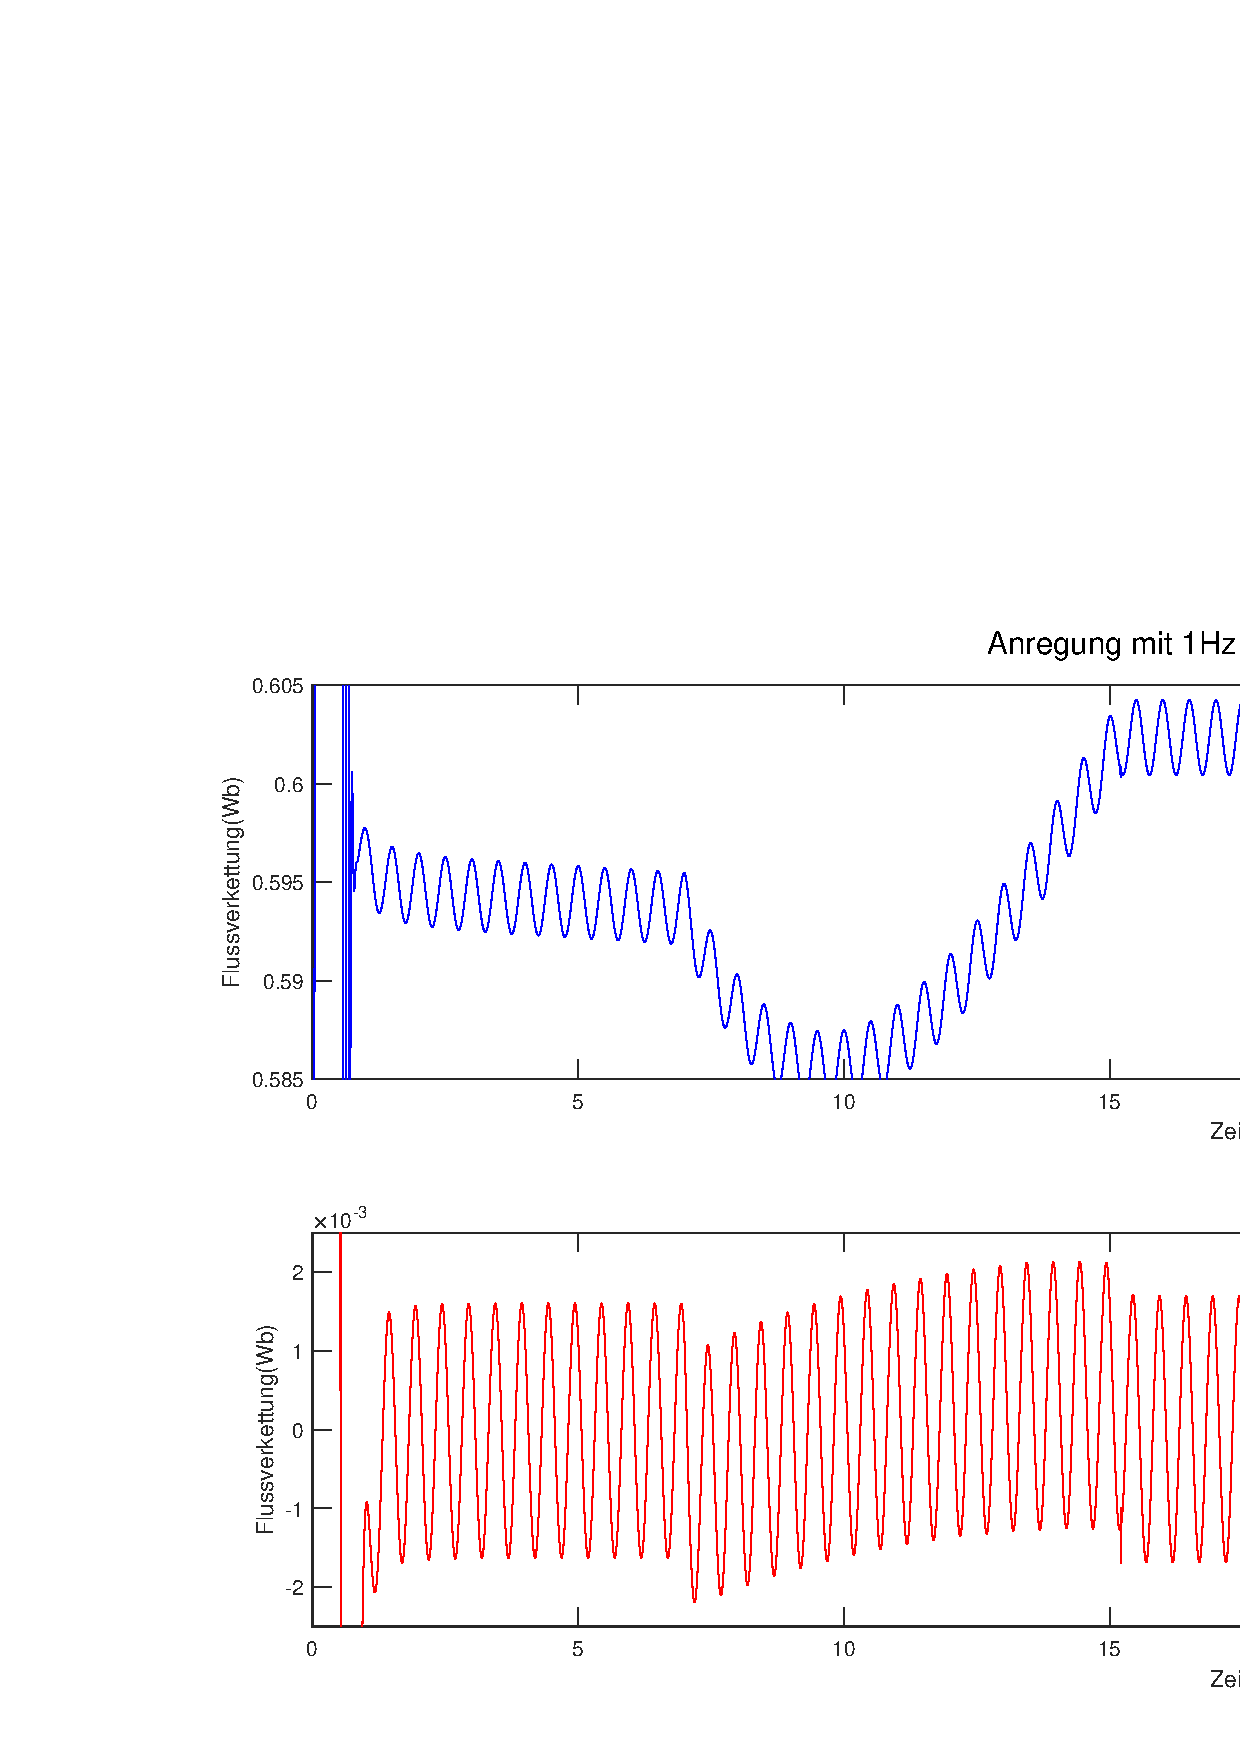
\includegraphics[scale=0.30]{Abbildungen/MRAS1.PNG}
	
\end{floatingfigure}
\vskip 0.4cm
\tiny{Das Ziel der Identifikation ist es, die Ausgaben zu Fehler des Modells gleich Null }\\
$\rightarrow e=y_{r}-y_{i}$=0 \\
\vskip 0.2cm
\tiny{Dieser Fehler des identifizierten Modells geht weiter in eine adaptiver Mechanismus, dessen Output bereits identifiziert.} 
\vskip 0.2cm
\tiny{Diese Methode ist iterativ bis die Fehler bis Null.\\ Normalerweise benutzt man einen Pi-Regler }\\
$\rightarrow F_{PI}(s)=K+\dfrac{1}{T_{i} \cdot s}$\\
\end{frame}
%%%%%%%%%%%%%%%%%%%%%%%%%%%%%%%%%%%%%%%%%%%%%%%%%%%%%%%%%%%%%%%%%%%%%%%%%
\begin{frame}
	\frametitle{Parameterschätzung der Flussverkettung durch MRAS}
	
	\vskip 0.2cm
	Umformen der Spannungsdifferentialgleichungen des PMSMs :\\
	\vskip 0.2cm
	$\frac{di_{q}}{dt}=\dfrac{1}{L_{q}}(U_{q}-R_{s}\cdot i_{q}-\omega \cdot L_{d}\cdot i_{d}-\omega \cdot \Psi_{f})$
	
	
	
	\begin{figure}[htbp]
		\centering
		\begin{minipage}[t]{0.48\textwidth}
			\centering
			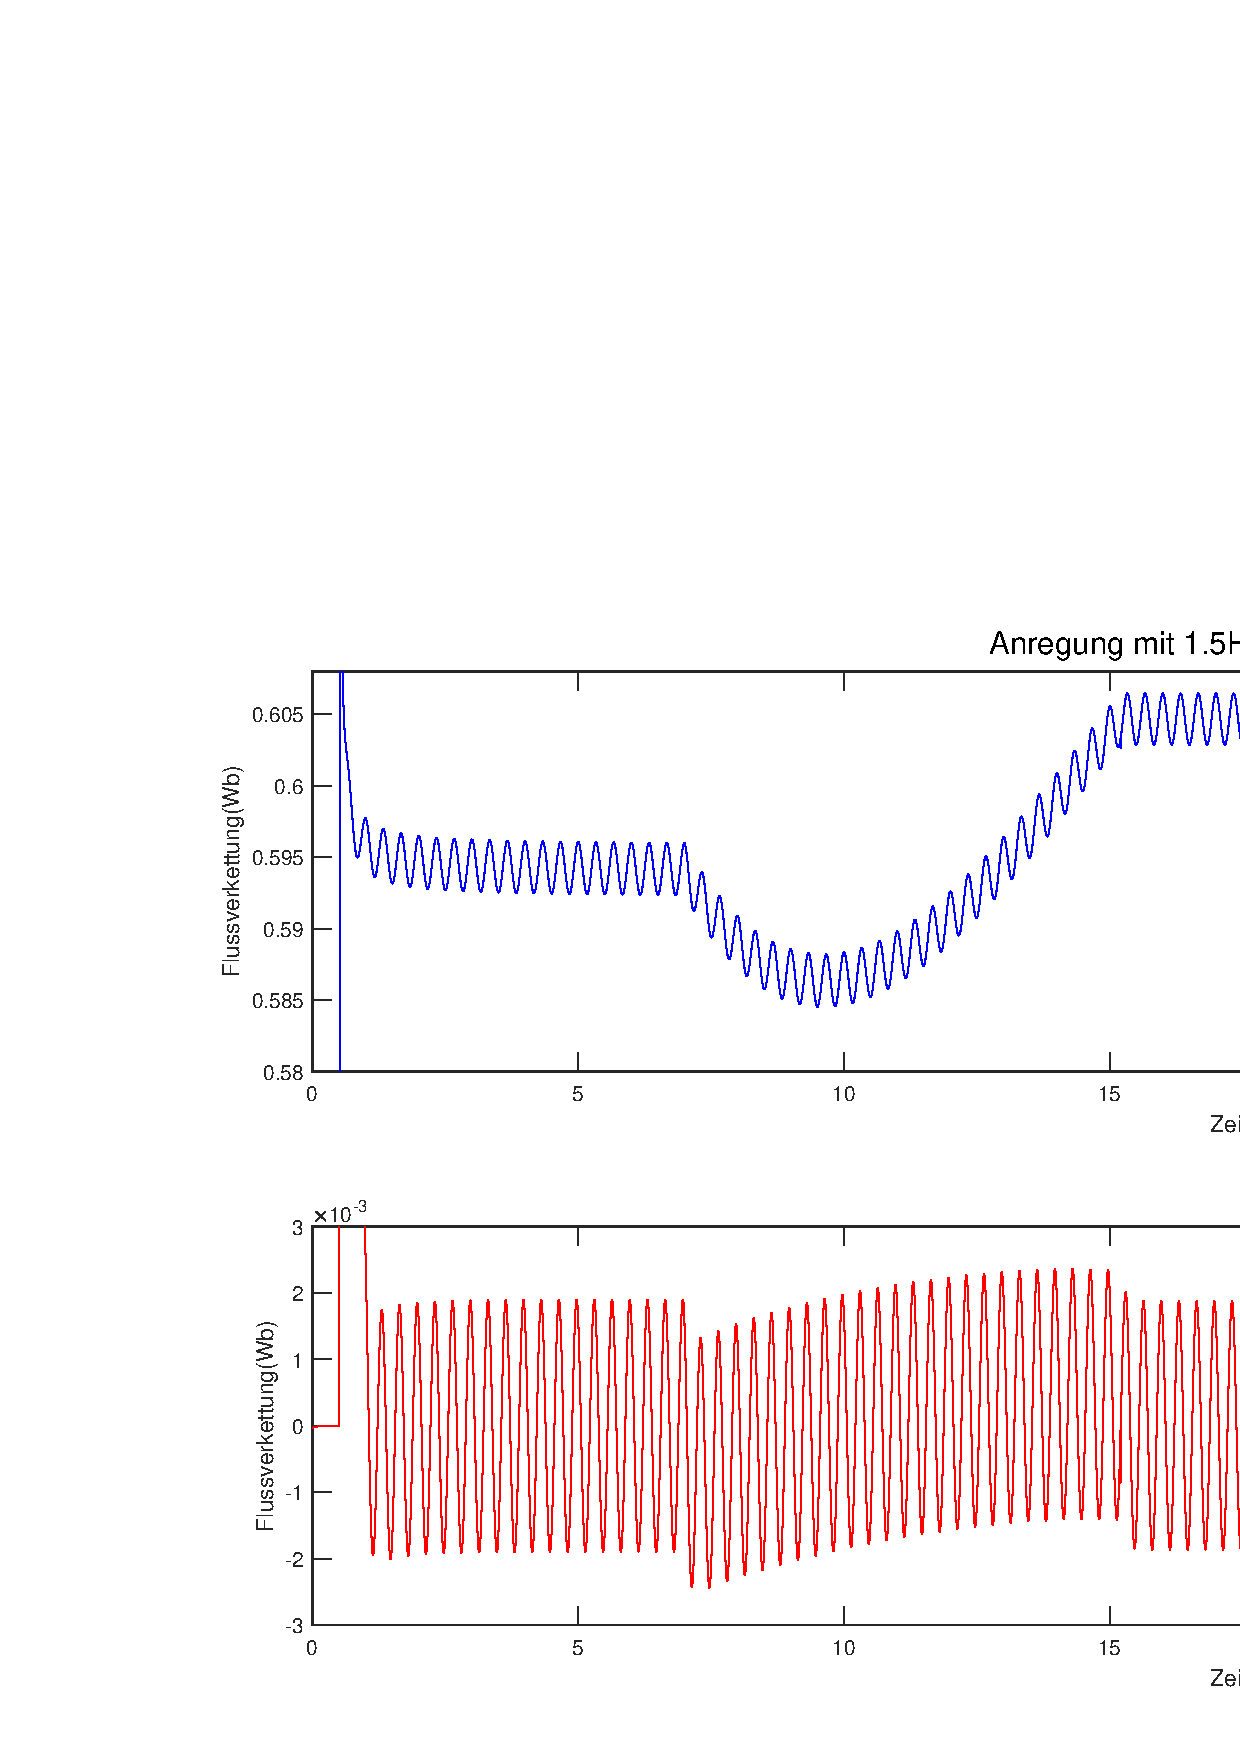
\includegraphics[width=5.4cm]{Abbildungen/MRAS2.PNG}
			
		\end{minipage}
		\begin{minipage}[t]{0.48\textwidth}
			\centering
			\includegraphics[width=6cm]{Abbildungen/MRAS3.JPG}
			
		\end{minipage}
	\end{figure}
	
\end{frame}
%%%%%%%%%%%%%%%%%%%%%%%%%%%%%%%%%%%%%%%%%%%%%%%%%%%%%%%%%%%%%%%%%%%%%%%%%
\begin{frame}
	\frametitle{Recursive Least Squares Method(RLS)}
	  
	\small{Durch ein lineares Modell mit den zu schätzenden Parametern $\hat{\theta}$ kann Ein- und Ausgangsdaten $Y=X\cdot\hat{\theta}$ verbindet werden.}\\
	\vskip 0.2cm
	$U_{q}=L_{q}\frac{di_{q}}{dt}+R_{s}i_{q}+\omega (L_{d}i_{d}+\Psi_{f})$\\
	$\stackrel{L_{q}=L_{d}=L_{s}}{\longrightarrow }\slashed{\frac{di_{q}}{dt}}+\omega \cdot i_{d}=-\frac{R_{s}}{L_{s}}\cdot i_{q}
	-\frac{\Psi_{f}}{L_{s}}\cdot\omega+\frac{U_{q}}{L_{s}}$\\
	\vskip 0.2cm
	\vskip 0.2cm
	$\omega\cdot i_{d}=\begin{bmatrix}
		-i_{q}&-\omega & U_{q}\\
	\end{bmatrix} \cdot \begin{bmatrix}
		\frac{R_{s}}{L_{s}}\\
		\frac{\Psi_{f}}{L_{s}}\\
		\frac{1}{L_{s}}
	\end{bmatrix}$\\
	\tiny{Messbare Eingangsdaten X=$\begin{bmatrix}
			-i_{q}&-\omega & U_{q}\\
		\end{bmatrix}$ eingeschätzte Parameters$\hat{\theta}=\begin{bmatrix}
			\frac{R_{s}}{L_{s}}\\
			\frac{\Psi_{f}}{L_{s}}\\
			\frac{1}{L_{s}}
	\end{bmatrix}$}
\end{frame}
%%%%%%%%%%%%%%%%%%%%%%%%%%%%%%%%%%%%%%%%%%%%%%%%%%%%%%%%%%%%%%%%%%%%%%%%%
\begin{frame}
\frametitle{RLS-Algorithmus}
 
\small{Die Formel für RLS erhält man wie folgt, wobei m Rekursionsschritt ist.} \\
\vskip 0.2cm
$\left\{\begin{array}{l} \gamma(m+1)=\frac{P_{m}X(m+1)}{\lambda+\mathbf{X(m+1)}^\intercal P_{m}X(m+1)}
\\
\\
	 \theta(m+1)= \theta(m)+\gamma(m+1) \cdot(Y(m+1)-\mathbf{X(m+1)}^\intercal \theta(m))
\\
\\
 P(m+1)=\frac{1}{\lambda}\cdot(P(m)-\gamma(m+1)\mathbf{X(m+1)}^\intercal P(m))
\end{array}\right.$\\
\vskip 0.2cm
$\lambda$:Vergessensfaktor$\longrightarrow$ die historischen Messdaten verlieren und die aktuellen Daten stärker gewichten(im Bereich 0.95$\textless\lambda\textless 1$)

\end{frame}
%%%%%%%%%%%%%%%%%%%%%%%%%%%%%%%%%%%%%%%%%%%%%%%%%%%%%%%%%%%%%%%%%%%%%%%%%
\begin{frame}
	\frametitle{Extended Kalman Filter(EKF)}
	 
	\small{ Ein mathematisches Verfahren zur iterativen Schätzung von Parametern zur Beschreibung von Systemzuständen auf der Basis von fehlerbehafteten Beobachtungen.}\\ 
	\vskip 0.2cm
	Die Systemzustandsraummodell und seine diskreten Messungen sind wie folgt beschrieben:
	$$\left\{\begin{array}{l}
		\Dot{x}=f[x(t)]+Bu(t)+\sigma(t) 
		\\y(t_{k})=h(t_{k})+\mu(t_{k})
	\end{array}\right.$$
	wobei $\sigma(t)$ und $\mu(t_{k})$ mittleres weißes Gaußsches Rauschen mit Kovarianz Q(t) bzw. $R(t_{k})$   sind.u(t) ist der Eingangsvektor.
\end{frame}

%%%%%%%%%%%%%%%%%%%%%%%%%%%%%%%%%%%%%%%%%%%%%%%%%%%%%%%%%%%%%%%%%%
\begin{frame}
	\frametitle{Variation der PMSM-Flussverkettung}
	  
	Um die Flussverkettung einzuschätzen, wird die als eine Zustandsvariable gewählt. Da die Flussverkettung kann sich nicht stark ändern, seine Ableitung wird auf Null gesetzt.\\
	\begin{floatingfigure}[r]{0.38\linewidth}
		\includegraphics[scale=0.46]{Abbildungen/Fluxdq.JPG}
		
	\end{floatingfigure}
	\vskip 0.2cm
	$$\left\{\begin{array}{l}
		\frac{di_{d}}{dt}=-\frac{R_{s}}{L_{d}}\cdot i_{d}+\frac{\omega L_{q}}{L_{d}}\cdot i_{q}+\frac{U_{d}}{L_{d}}+\frac{\omega}{L_{d}}\cdot \psi_{rq}\\ \frac{di_{q}}{dt}=-\frac{R_{s}}{L_{q}}\cdot i_{q}-\frac{\omega L_{d}}{L_{q}}\cdot i_{d}+\frac{U_{q}}{L_{q}}-\frac{\omega}{L_{q}}\cdot \psi_{rd}
		\\\frac{\psi_{rd}}{dt}=0\\
		\frac{\psi_{rq}}{dt}=0\\
	\end{array}\right.$$
	
\end{frame}
%%%%%%%%%%%%%%%%%%%%%%%%%%%%%%%%%%%%%%%%%%%%%%%%%%%%%%%%%%%%%%%%%%
\begin{frame}
	\frametitle{Kalman-Filter vierter Ordnung}
	
	$\Dot{x}=f[x(t)]+Bu(t)+\sigma(t)$\\
	\vskip 0.2cm
	f[x(t)]=$\begin{bmatrix}
		f(1)\\
		f(2)\\
		f(3)\\
		f(4)
	\end{bmatrix}$
	=$\begin{bmatrix}
		-\frac{R_{s}}{L_{d}}\cdot i_{d}+\frac{\omega L_{q}}{L_{d}}\cdot i_{q}+\frac{\omega}{L_{d}}\cdot \psi_{rq}\\
		-\frac{R_{s}}{L_{q}}\cdot i_{q}-\frac{\omega L_{d}}{L_{q}}\cdot i_{d}-\frac{\omega}{L_{q}}\cdot \psi_{rd}\\
		0\\
		0
	\end{bmatrix}$
	B=$\begin{bmatrix}
		\frac{1}{L_{d}} & 0\\
		0 &\frac{1}{L_{q}}\\
		0 &0\\
		0 &0
	\end{bmatrix}$
	$y(t_{k})=h(t_{k})+\mu(t_{k})$
	\vskip 0.2cm
	$h(t_{k})=\begin{bmatrix}
		i_{d}\\
		i_{q}
	\end{bmatrix}$\\
	
	Zustandsgrö{\ss}e x=$\begin{bmatrix}
		
		i_{d}&i_{q}&\psi_{rd}&\psi_{rq}\\
		
	\end{bmatrix}^T$\\
	Eingangsgrö{\ss}e  u=$\begin{bmatrix}
		
		U_{d}&U_{q}\\
		
	\end{bmatrix}^T$
	
\end{frame}
%%%%%%%%%%%%%%%%%%%%%%%%%%%%%%%%%%%%%%%%%%%%%%%%%%%%%%%%%%%%%%%%%%%%%%%%%
\begin{frame}
	\frametitle{Die Jacobi-Matrizen definieren}
	 
	Jacobian Matrix: Partielle Ableitung nach den Zustandsgrö{\ss}e x\\
    \vskip 0.2cm
	F(x(t))=$\frac{\partial f}{\partial x}\bigg|_{x = x(t)}  =\begin{bmatrix}
		-\frac{R_{s}}{L_{d}} & \frac{\omega L_{q}}{L_{d}}& 0 &\frac{\omega }{L_{d}} \\
		-\frac{\omega L_{d}}{L_{q}} & -\frac{R_{s}}{L_{q}} &-\frac{\omega} {L_{q}} & 0 \\
		0 & 0 & 0 &0\\
		0 & 0 & 0 &0
	\end{bmatrix}$
	\vskip 0.2cm
	H(x(t))=$\frac{\partial h}{\partial x}\bigg|_{x = x(t)}  =\begin{bmatrix}
		
		1 & 0 & 0 &0\\
		0 & 1 & 0 &0
	\end{bmatrix}$
\end{frame}
%%%%%%%%%%%%%%%%%%%%%%%%%%%%%%%%%%%%%%%%%%%%%%%%%%%%%%%%%%%%%%%%%%
\begin{frame}
	\frametitle{Algorithmus des EKFs}
	
	\small{Sowohl der optimale Zustand als auch seine Kovarianz $P_{k|k}$ werden berechnet
		in einer zweistufigen Schleife}
	\begin{figure}[htbp]
		\centering
		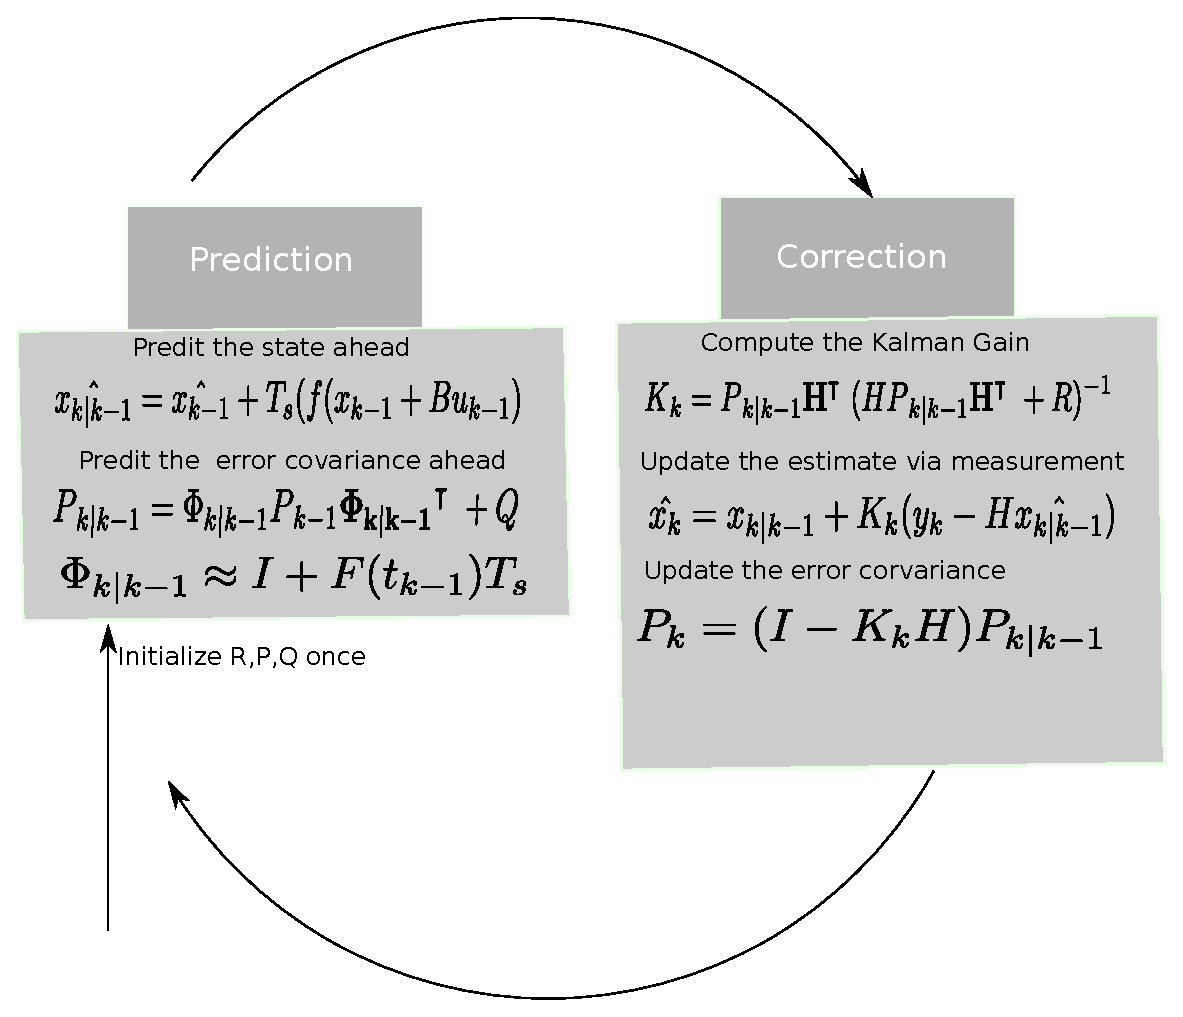
\includegraphics[scale=0.33]{Abbildungen/EKF.eps}
		
	\end{figure}	
	
	
\end{frame}
%%%%%%%%%%%%%%%%%%%%%%%%%%%%%%%%%%%%%%%%%%%%%%%%%%%%%%%%%%%%%%%%%%
\begin{frame}
	\frametitle{Luenberger Beobachter(LB)}
	  
	\tiny{Ein Beobachter ist ein System, das aus bekannten Eingangsgrößen und Ausgangsgrößen eines beobachteten Referenzsystems nicht messbare Größen (Zustände) rekonstruiert. Dazu bildet er das beobachtete Referenzsystem als Modell nach und führt mit einem Regler die messbaren und deshalb mit dem Referenzsystem vergleichbaren.}\\
	\vskip 0.2cm
	Der Zustandsbeobachter ist gegeben durch\\
	$\dot{\hat{x}}=Ax+Bu+K(y-\hat{y})$\\
	$\hat{y}=C\hat{x}$
	
	\begin{figure}[htbp]
		\centering
		\includegraphics[scale=0.35]{Abbildungen/Luenberger state observert.png}
		
	\end{figure}	
\end{frame}
%%%%%%%%%%%%%%%%%%%%%%%%%%%%%%%%%%%%%%%%%%%%%%%%%%%%%%%%%%%%%%%%%%
\begin{frame}
	\frametitle{Luenberger Beobachter vierter Ordnung}
	  
	\tiny{Die Spannungsgleichung auf der $\alpha–\beta$-Koordinate kann
		beschrieben werden:}\\
	\vskip 0.2cm
	$\begin{bmatrix}
		u_{\alpha}\\
		u_{\beta}
	\end{bmatrix}$=$\begin{bmatrix}
		R_{s}+\frac{d}{dt}L_{q}&0\\
		0 & R_{s}+\frac{d}{dt}L_{q}
	\end{bmatrix}$ $\begin{bmatrix}
		i_{\alpha}\\
		i_{\beta}
	\end{bmatrix}$+$\begin{bmatrix}
		e_{\alpha}\\
		e_{\beta}
	\end{bmatrix}$ wobei $e_{\alpha}=-\psi\omega\sin(\theta_{e})$,
	$e_{\beta}=\psi\omega\cos(\theta_{e})$\\
	\vskip 0.2cm
	$e_{\alpha}$ und $e_{\beta}$ sind die Back-EMF auf der festen Koordinate. Die Back-EMF von PMSM kann nicht direkt gemessen werden und daher benutzt man einen Luenberger Beobachter.\\
	$$\left\{\begin{array}{l}
		\frac{di_{\alpha}}{dt}=-\frac{R_{s}}{L_{q}}i_{\alpha}-\frac{e_{\alpha}}{L_{q}}+\frac{U_{\alpha}}{L_{q}}
		\\\frac{di_{\beta}}{dt}=-\frac{R_{s}}{L_{q}}i_{\beta}-\frac{e_{\beta}}{L_{q}}+\frac{U_{\beta}}{L_{q}}\\
		\frac{de_{\alpha}}{dt}=\omega e_{\beta}\\
		\frac{de_{\beta}}{dt}=-\omega e_{\alpha}
	\end{array}\right.$$
	$\dot{\hat{x}}=Ax+Bu+K(y-\hat{y})$\\
	\vskip 0.2cm
	x=$\begin{bmatrix}
		i_{\alpha} \\ 
		i_{\beta}\\  
		e_{\alpha} \\
		e_{\beta}  \\
	\end{bmatrix}$u=$\begin{bmatrix}
		U_{\alpha} \\ 
		U_{\beta}\\  
	\end{bmatrix}$A=$\begin{bmatrix}
		-\frac{R_{s}}{L_{q}} & 0 & -\frac{1}{L_{q}}&0\\ 
		0 & -\frac{R_{s}}{L_{q}}&0 &-\frac{1}{L_{q}}\\  
		0 & 0 & 0 &\omega \\
		0 & 0 & -\omega &0 \\
	\end{bmatrix}$ B=$\begin{bmatrix}
		\frac{1}{L_{q}}& 0 \\ 
		0 & \frac{1}{L_{q}}\\  
		0 & 0  \\
		0 & 0  \\
	\end{bmatrix}$ K=$\begin{bmatrix}
		K1& 0 \\ 
		0 & K1\\  
		K2& 0  \\
		0 & K2  
	\end{bmatrix}$
\end{frame}
%%%%%%%%%%%%%%%%%%%%%%%%%%%%%%%%%%%%%%%%%%%%%%%%%%%%%%%%%%%%%%%%%%
\begin{frame}
	\frametitle{BSB zur Schätzung der Flussverkettung durch LB}
	
	$\hat{y}=C\hat{x}$
	$\hat{y}$=$\begin{bmatrix}
		i_{\alpha}\\ 
		i_{\beta}\\  
		
	\end{bmatrix}$ C=$\begin{bmatrix}
		1& 0 & 0 & 0 \\ 
		0& 1 & 0 & 0  
		
	\end{bmatrix}$
	
	\begin{figure}[htbp]
		\centering
		\includegraphics[scale=0.35]{Abbildungen/Luenberger Obsever.png}
		
	\end{figure}	
\end{frame}

%%%%%%%%%%%%%%%%%%%%%%%%%%%%%%%%%%%%%%%%%%%%%%%%%%%%%%%%%%%%%%%%%%
	\section{Ergebnis von Simulink}
	\begin{frame}
		\frametitle{Parameterschätzung $\psi_{f}  $ ohne Verschiebung}
		
		\begin{figure}[htbp]
			\centering
			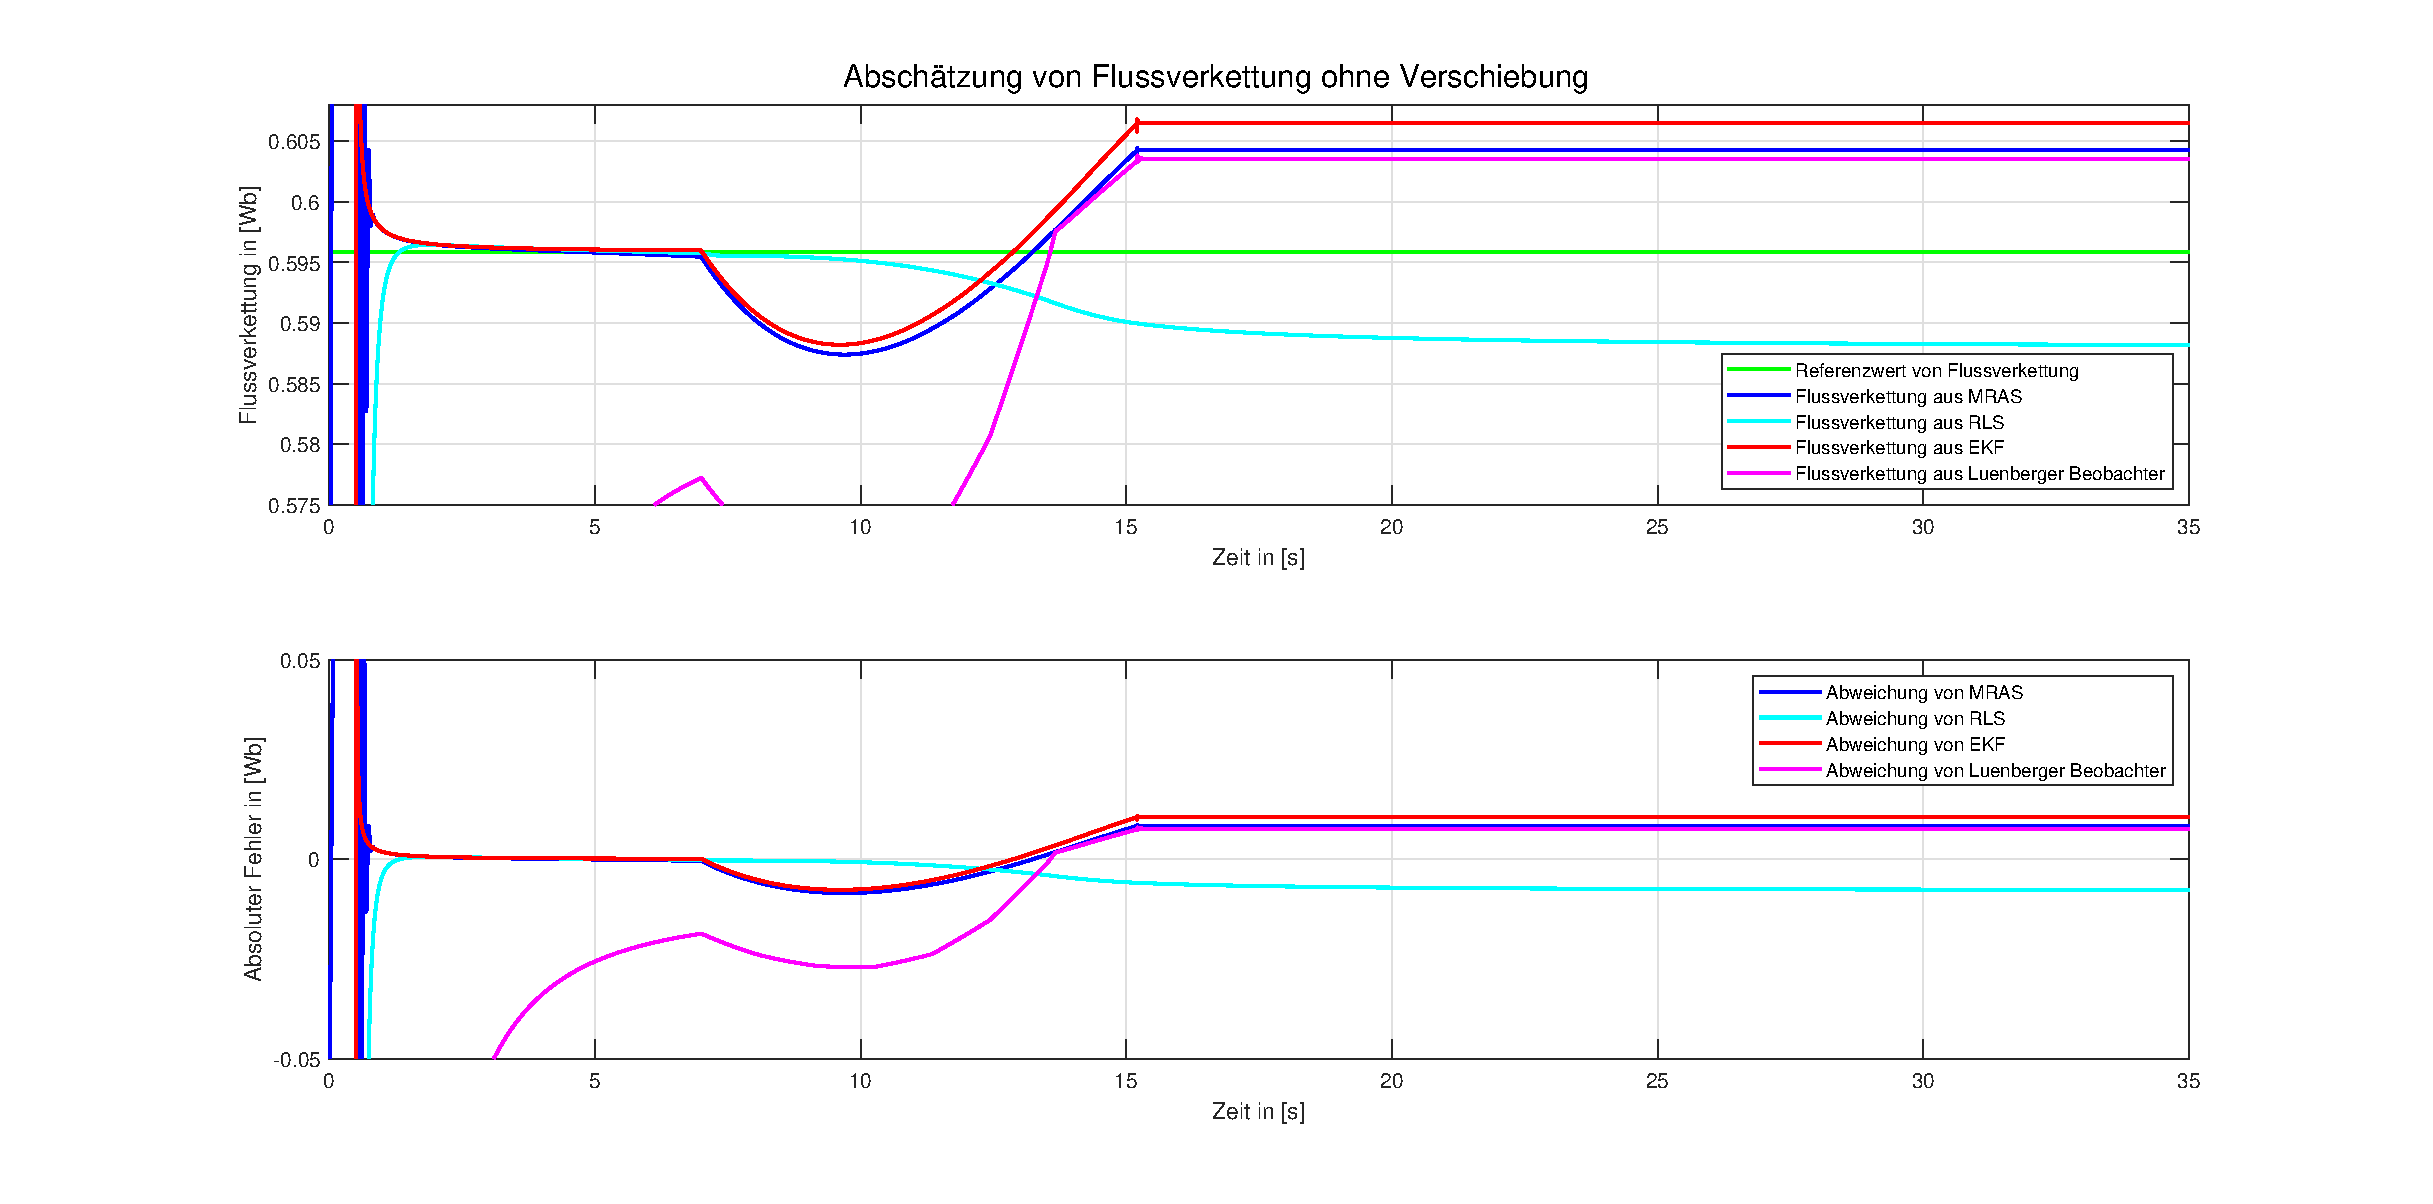
\includegraphics[scale=0.30]{Abbildungen/OhneVerschiebung.eps}
			
		\end{figure}	
		
	\end{frame}
%%%%%%%%%%%%%%%%%%%%%%%%%%%%%%%%%%%%%%%%%%%%%%%%%%%%%%%%%%%%%%%%%%
\begin{frame}
	\frametitle{Drehzahl und Drehmoment bis statischer Betriebsfall}
	
	\begin{figure}[htbp]
		\centering
		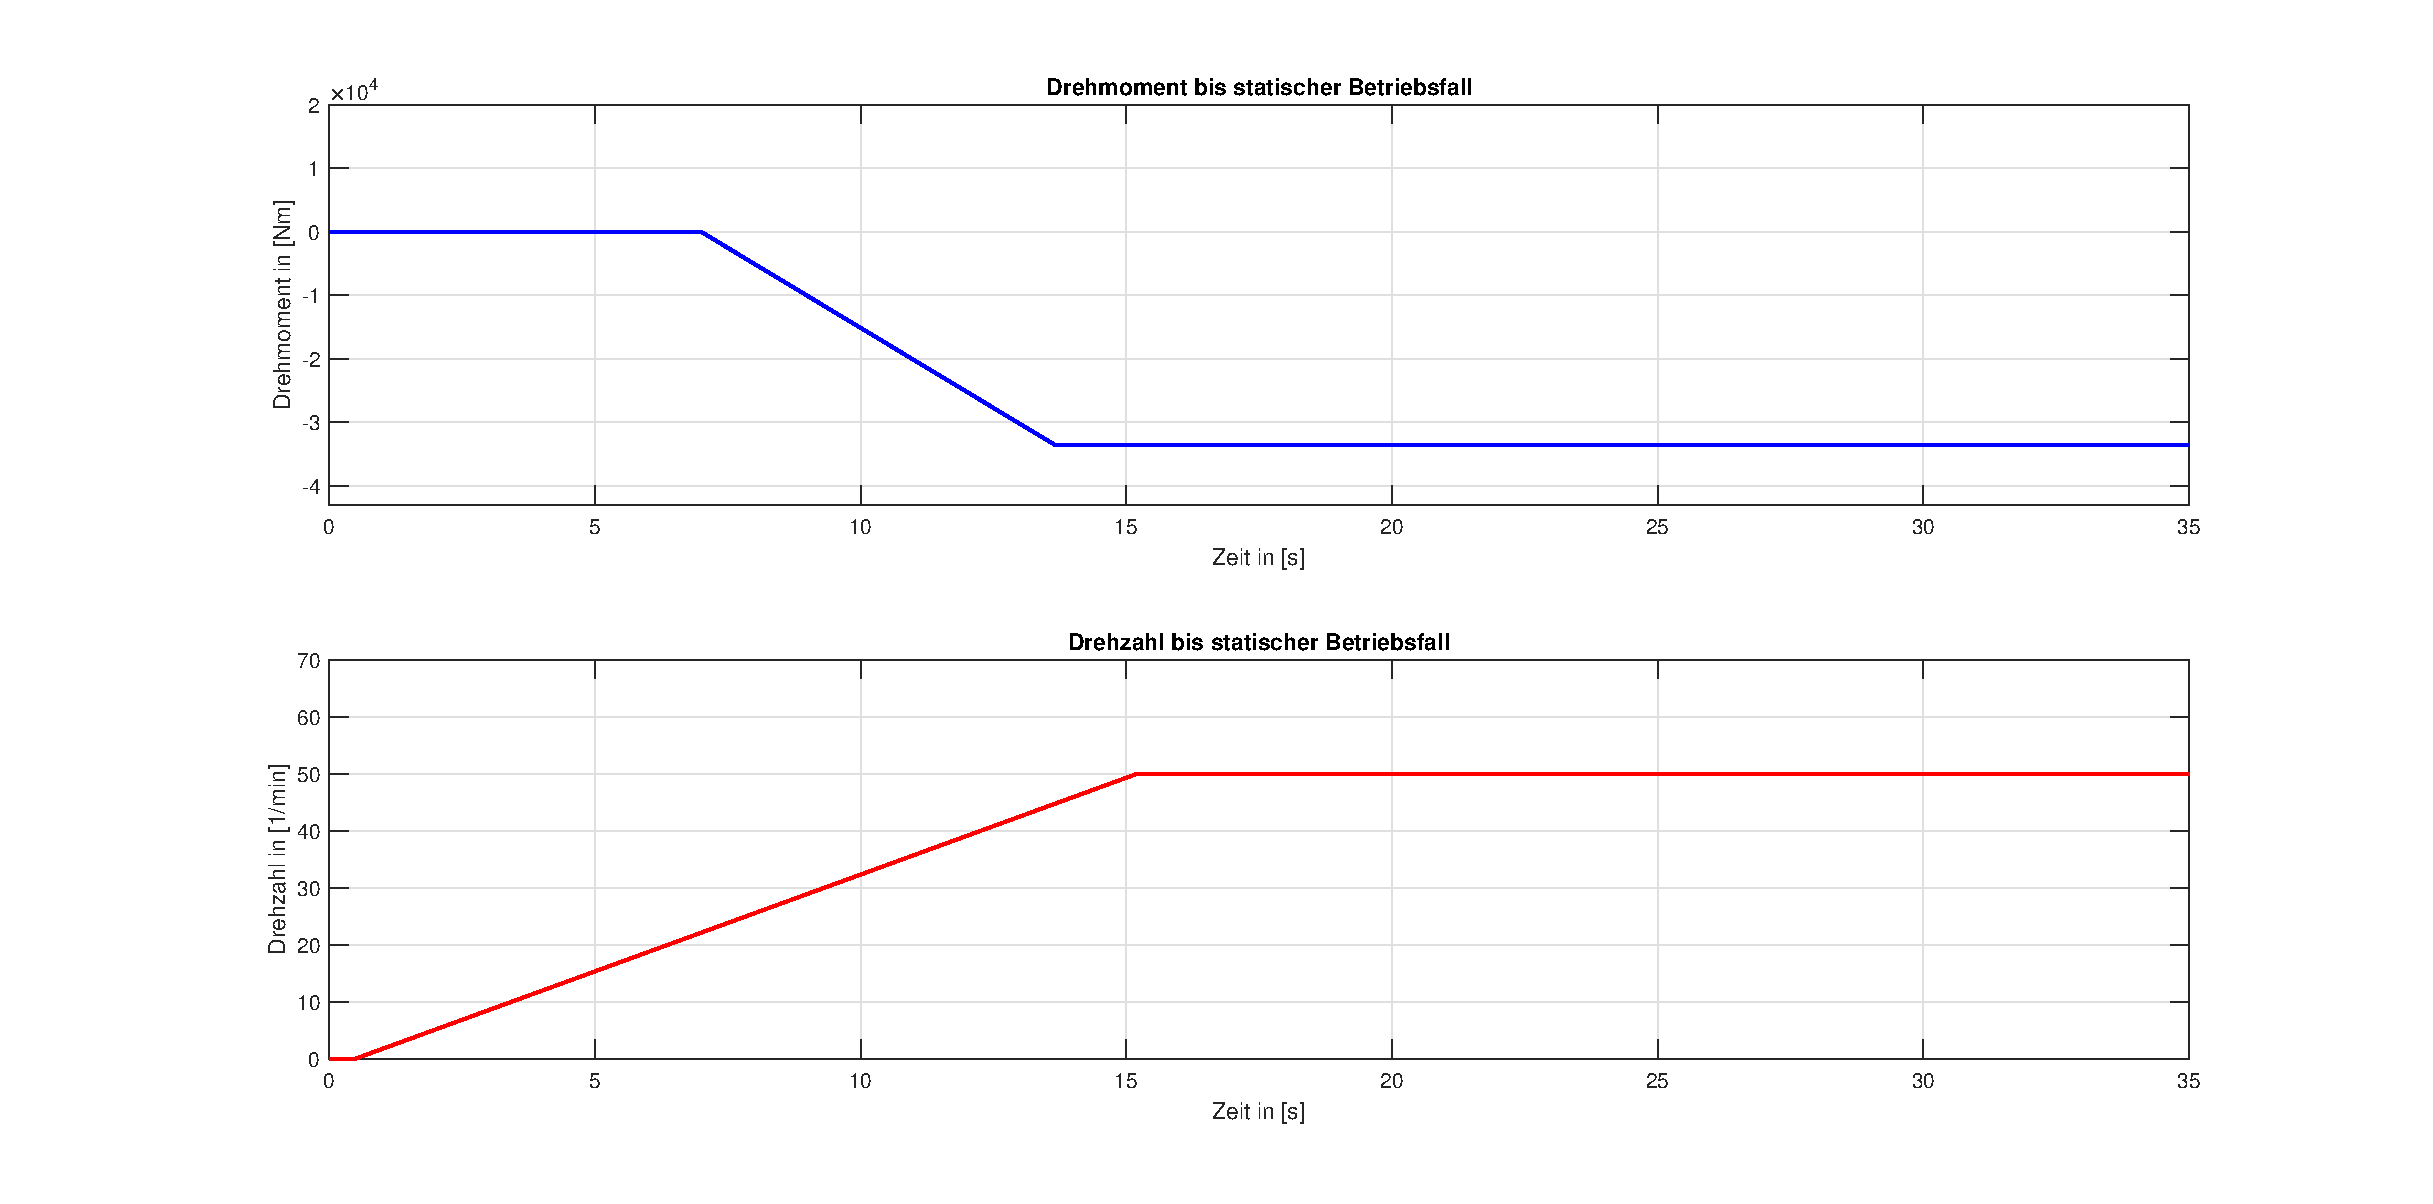
\includegraphics[scale=0.30]{Abbildungen/DrehmomentDrehzahl.eps}
		
	\end{figure}	
	
\end{frame}
%%%%%%%%%%%%%%%%%%%%%%%%%%%%%%%%%%%%%%%%%%%%%%%%%%%%%%%%%%%%%%%%%%%%%%%%%
\begin{frame}
	\frametitle{Vergleich MRAS und EKF ber der Anregung mit 0.1Hz sinusförmiger Schwingung}
	 
	\begin{figure}[htbp]
		\centering
		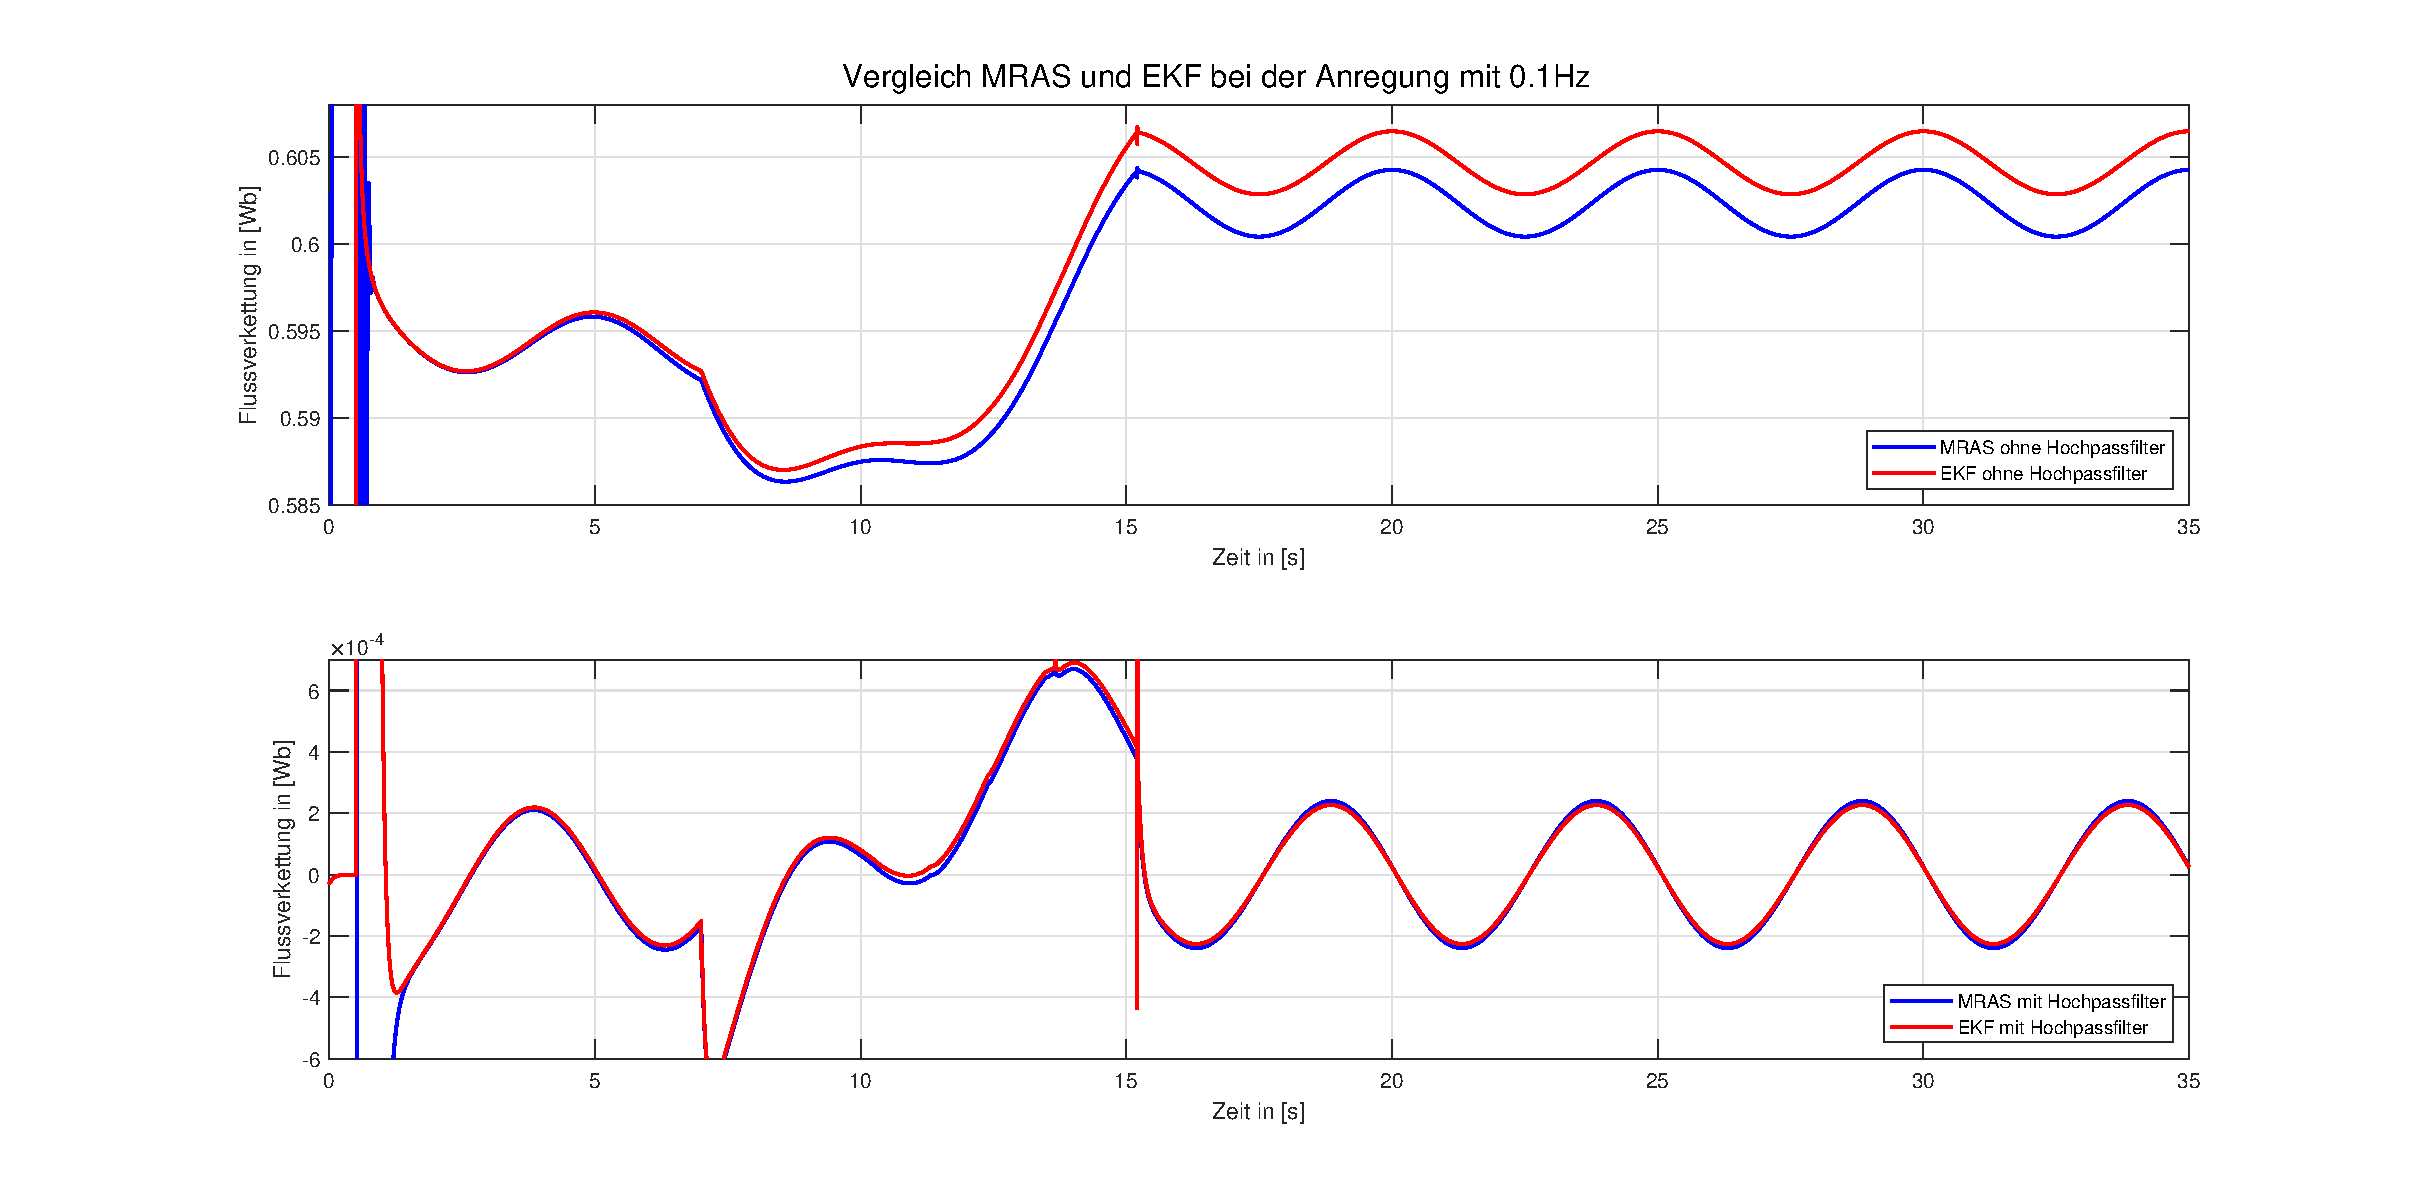
\includegraphics[scale=0.30]{Abbildungen/Vergleich_01Hz.eps}
		
	\end{figure}	
	
\end{frame}
%%%%%%%%%%%%%%%%%%%%%%%%%%%%%%%%%%%%%%%%%%%%%%%%%%%%%%%%%%%%%%%%%%%%%%%%%
\begin{frame}
	\frametitle{Vergleich MRAS und EKF ber der Anregung mit 1Hz sinusförmiger Schwingung }
	
	\begin{figure}[htbp]
		\centering
		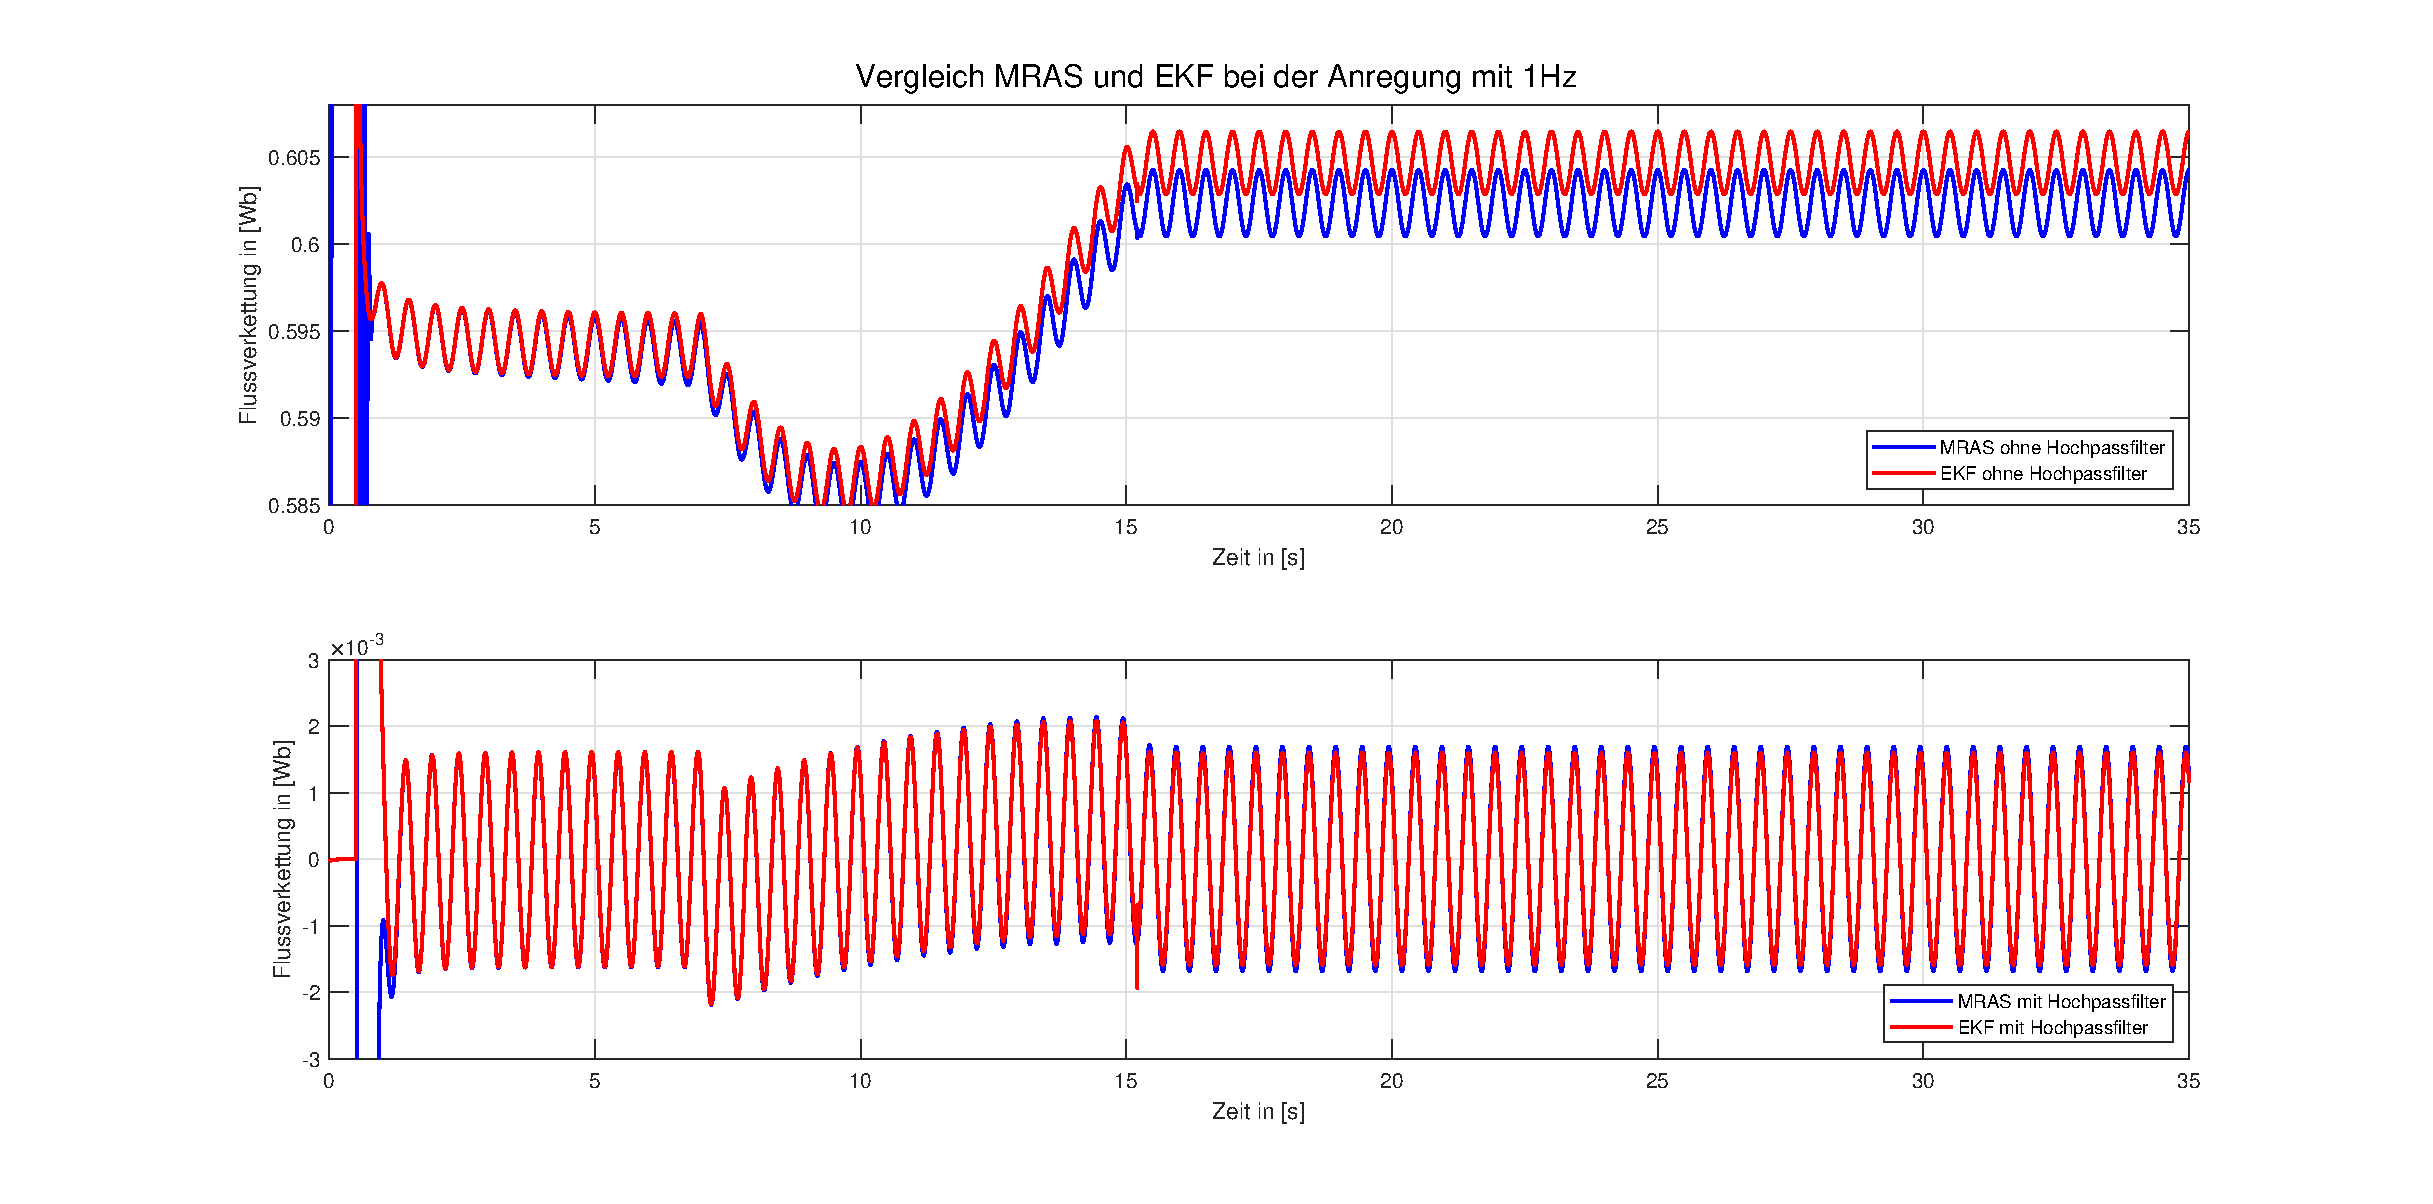
\includegraphics[scale=0.30]{Abbildungen/Vergleich_1Hz.eps}
		
	\end{figure}	
	
\end{frame}
%%%%%%%%%%%%%%%%%%%%%%%%%%%%%%%%%%%%%%%%%%%%%%%%%%%%%%%%%%%%%%%%%%%%%%%%%
\begin{frame}
	\frametitle{Vergleich MRAS und EKF ber der Anregung mit 1Hz sinusförmiger Schwingung im Zeitraum 20s bis 25s }
	
	\begin{figure}[htbp]
		\centering
		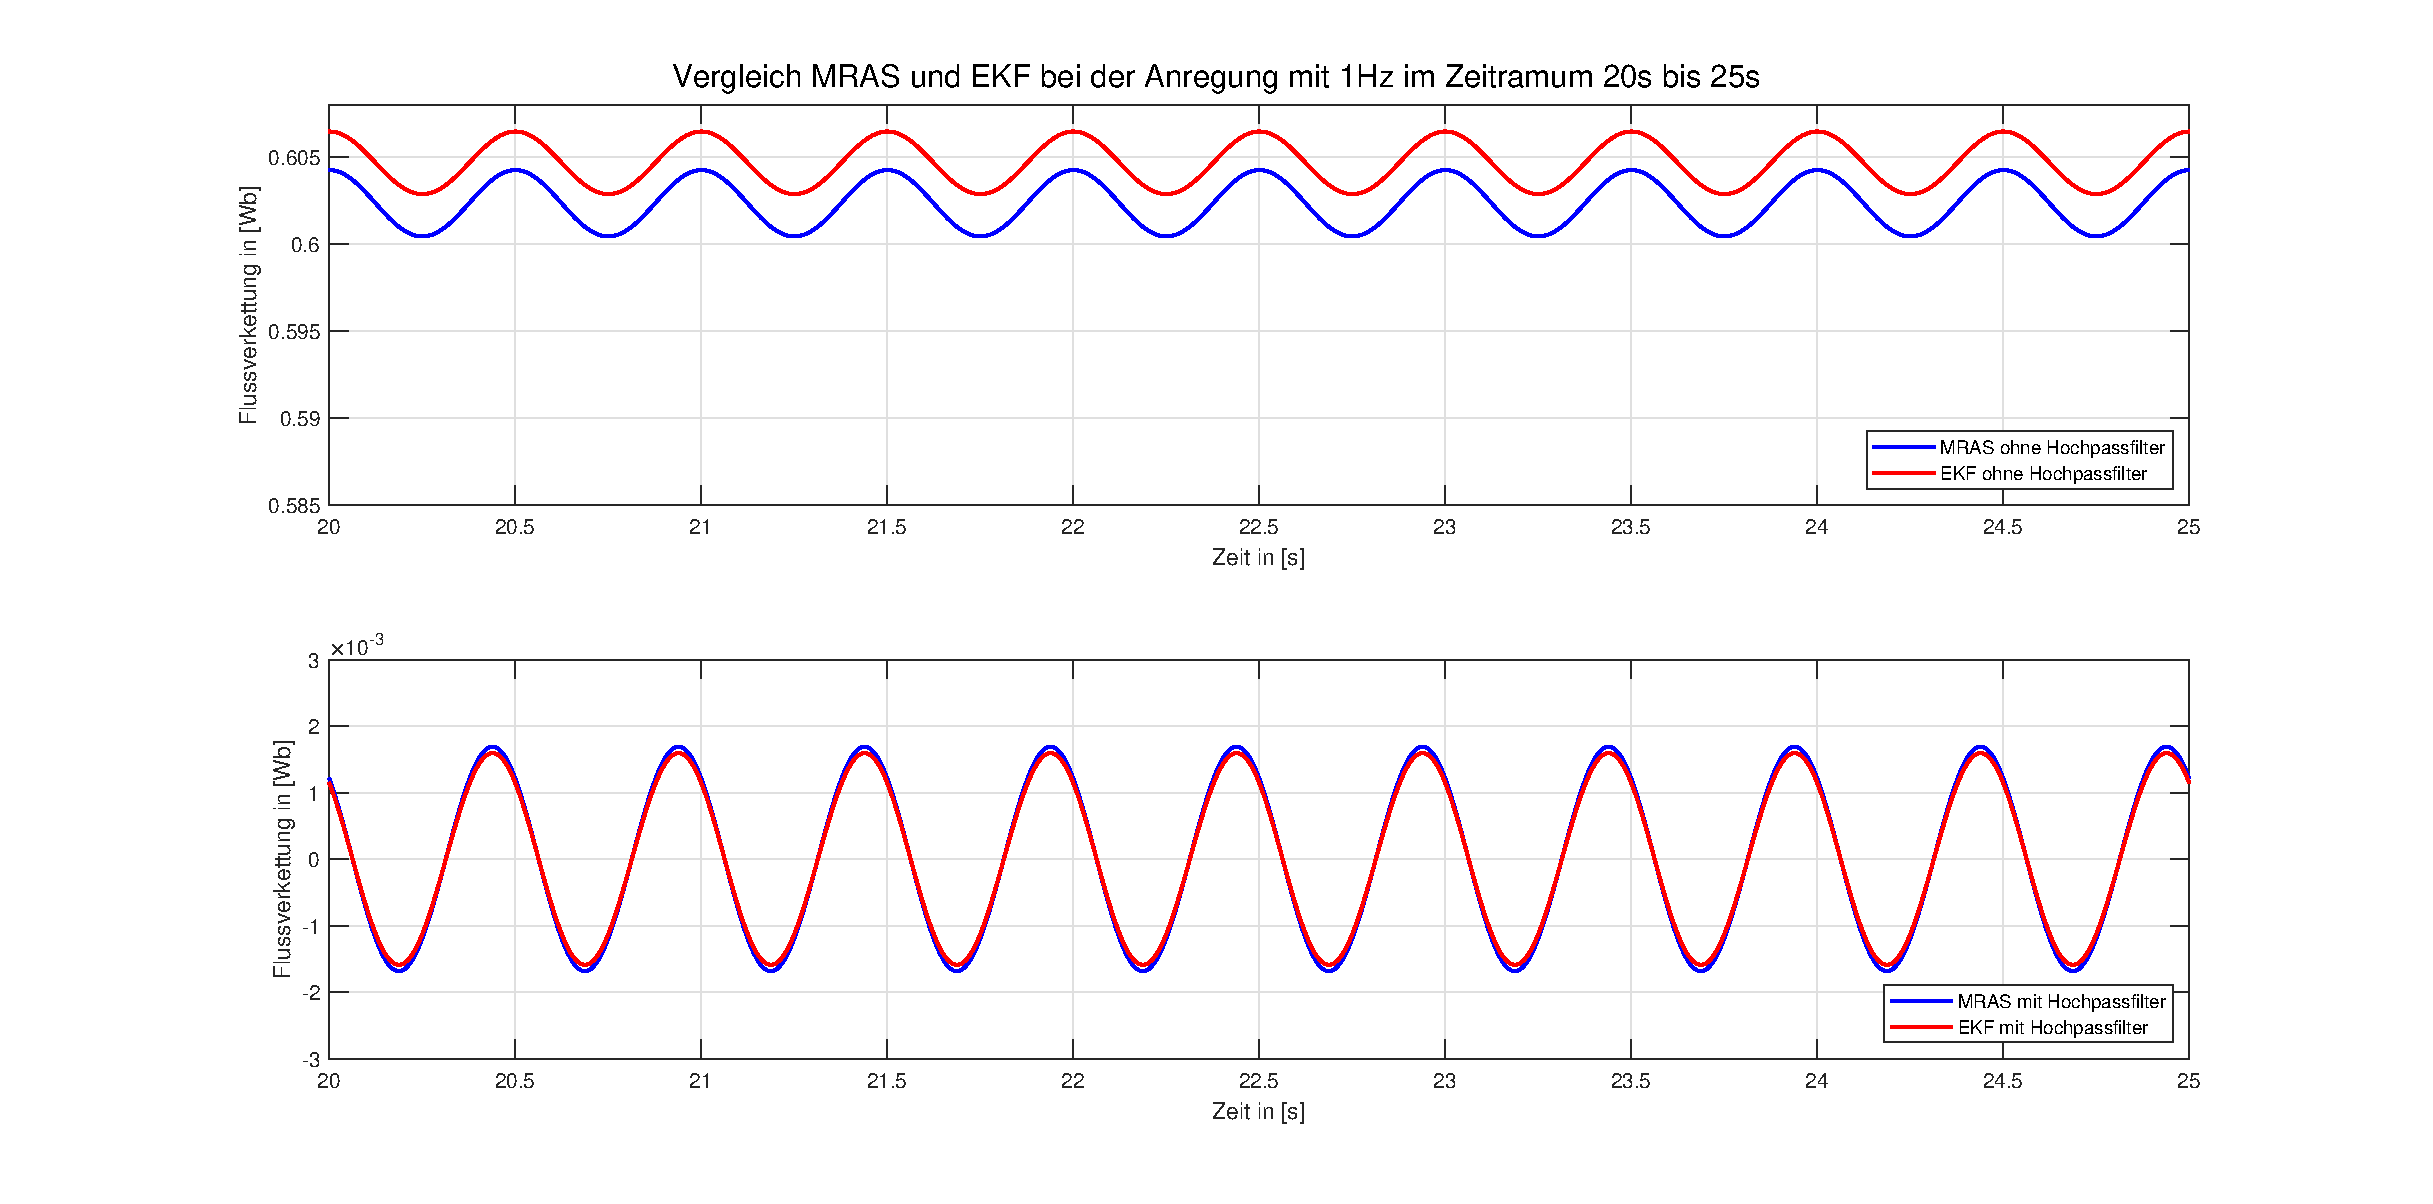
\includegraphics[scale=0.30]{Abbildungen/Vergleich_1Hz_20s.eps}
		
	\end{figure}	
	
\end{frame}
%%%%%%%%%%%%%%%%%%%%%%%%%%%%%%%%%%%%%%%%%%%%%%%%%%%%%%%%%%%%%%%%%%%%%%%%%
\begin{frame}
	\frametitle{Vergleich MRAS und EKF ber der Anregung mit 2Hz sinusförmiger Schwingung }
	
	\begin{figure}[htbp]
		\centering
		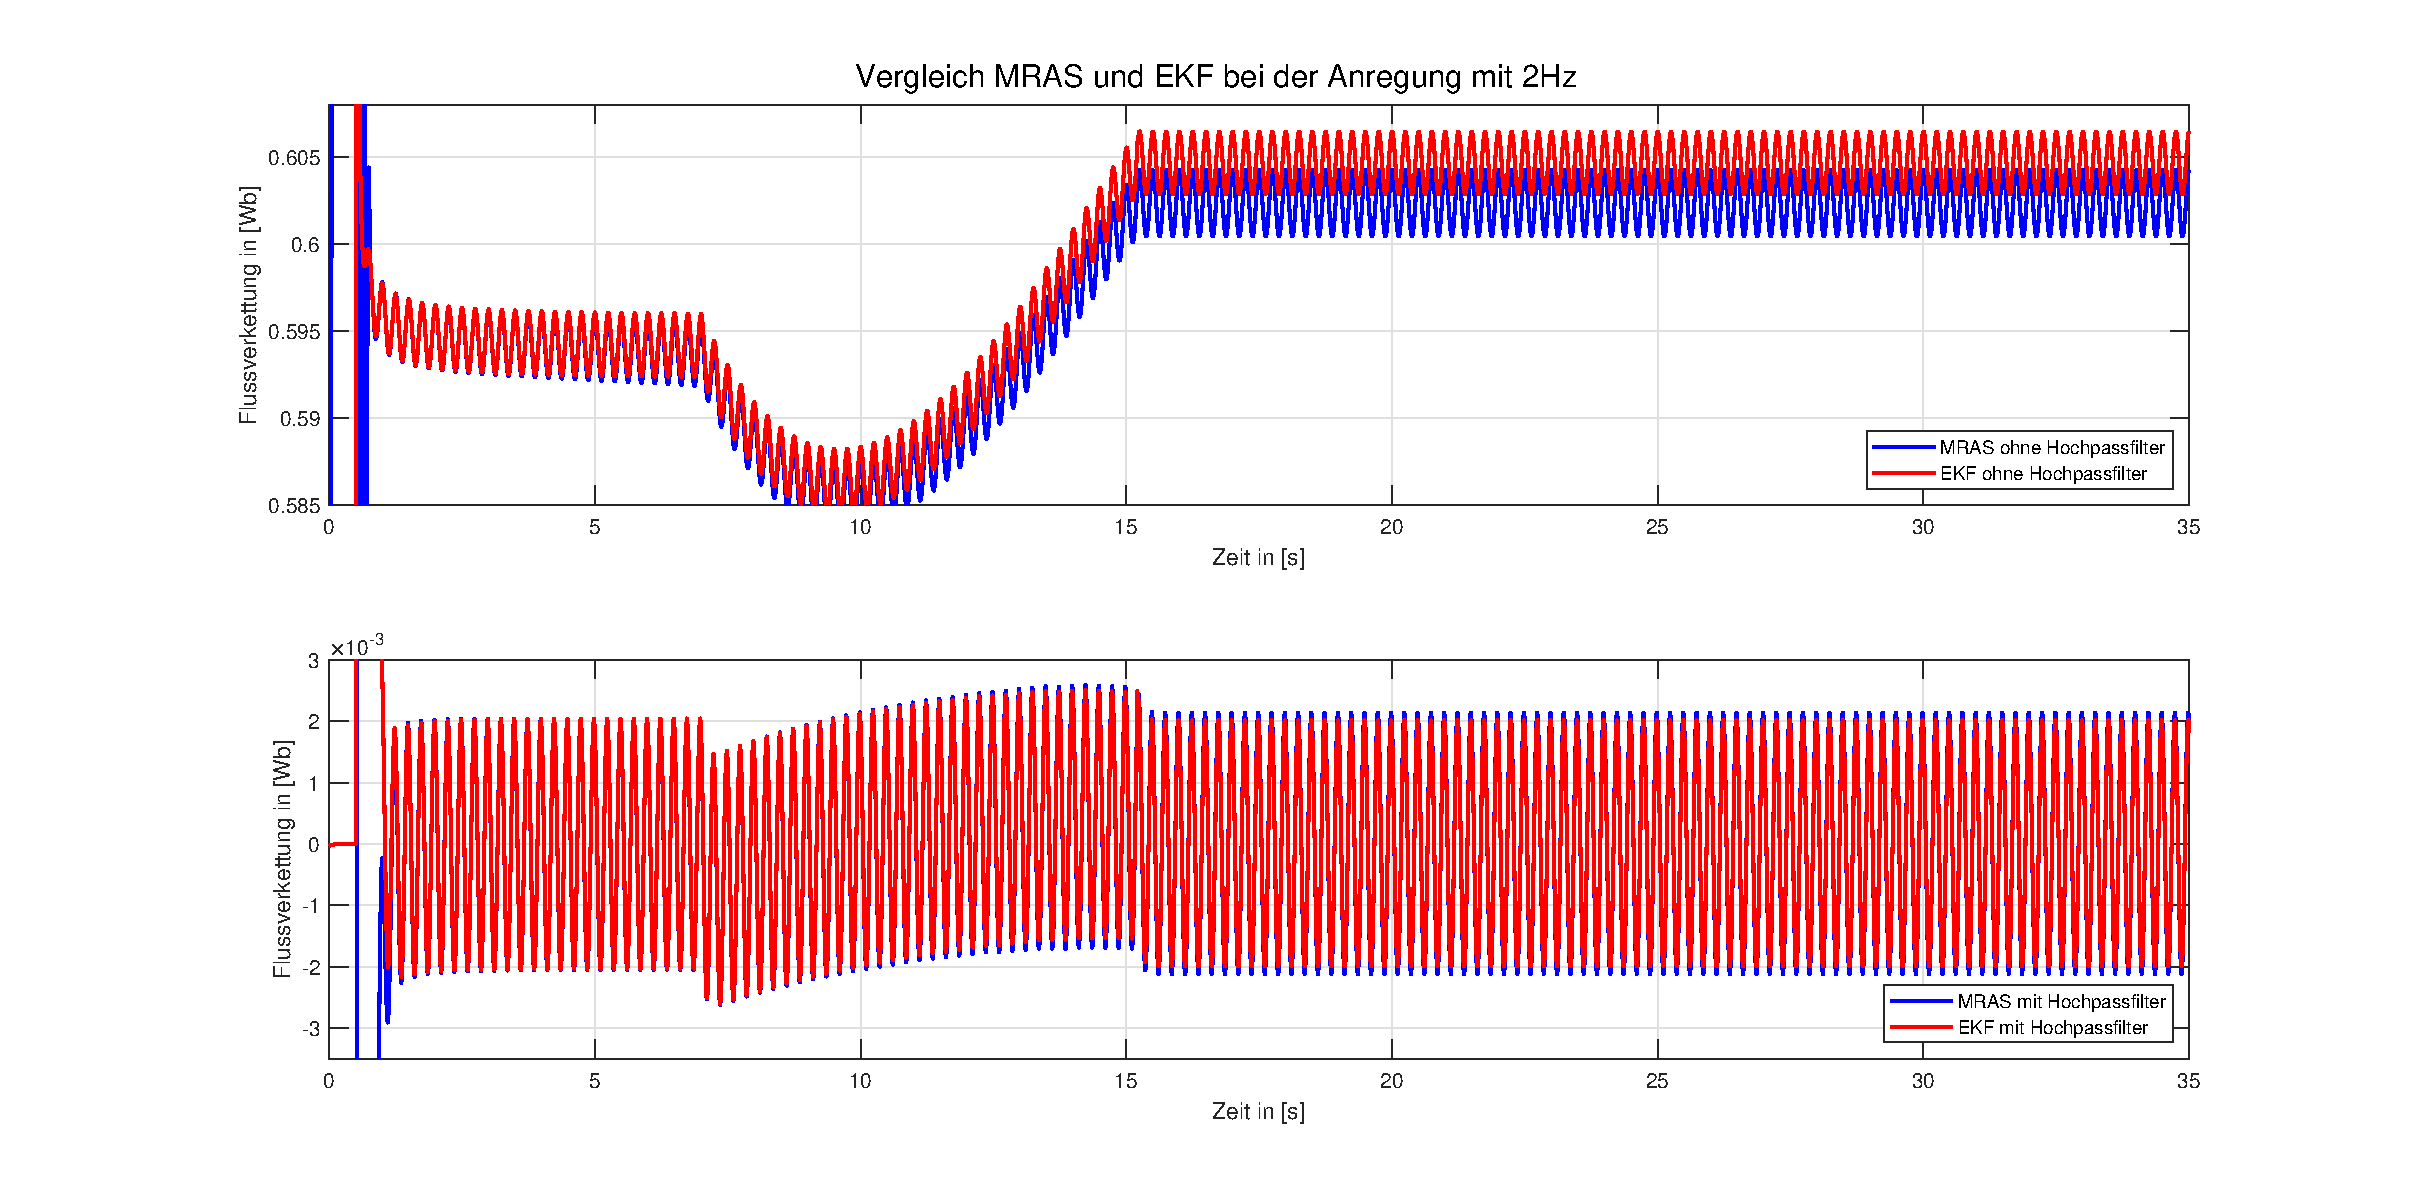
\includegraphics[scale=0.30]{Abbildungen/Vergleich_2Hz.eps}
		
	\end{figure}	
	
\end{frame}
%%%%%%%%%%%%%%%%%%%%%%%%%%%%%%%%%%%%%%%%%%%%%%%%%%%%%%%%%%%%%%%%%%%%%%%%%
\begin{frame}
	\frametitle{Vergleich MRAS und EKF ber der Anregung mit 2Hz sinusförmiger Schwingung im Zeitraum 20s bis 25s }
	
	\begin{figure}[htbp]
		\centering
		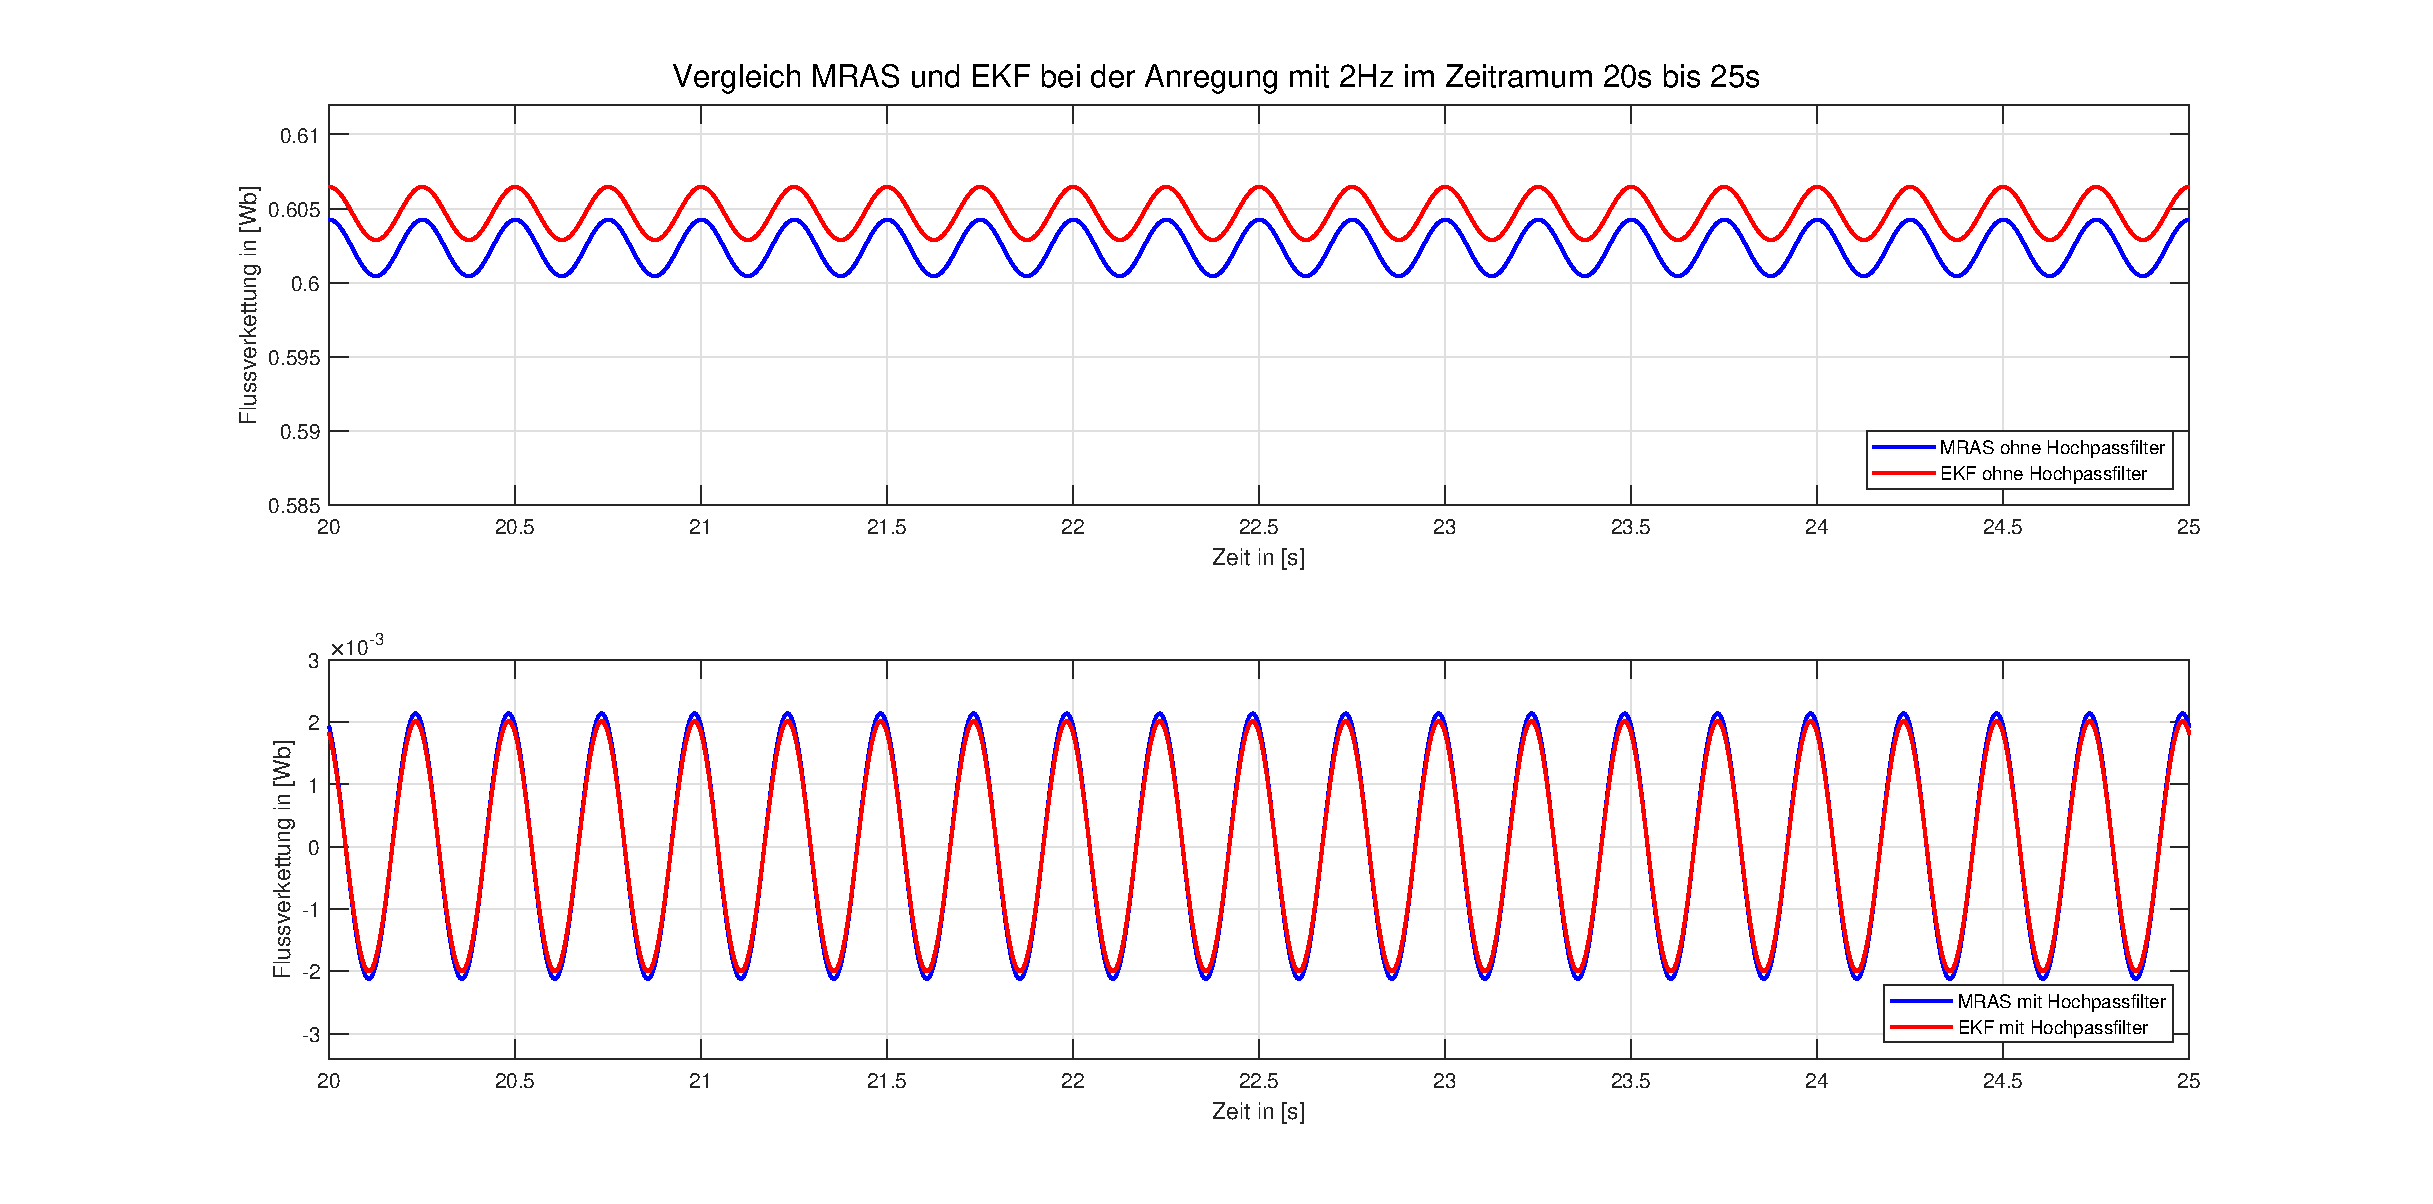
\includegraphics[scale=0.30]{Abbildungen/Vergleich_2Hz_20s.eps}
		
	\end{figure}	
	
\end{frame}
%%%%%%%%%%%%%%%%%%%%%%%%%%%%%%%%%%%%%%%%%%%%%%%%%%%%%%%%%%%%%%%%%%%%%%%%%
\begin{frame}
	\frametitle{Vergleich MRAS und EKF ber der Anregung mit 5Hz sinusförmiger Schwingung }
	
	\begin{figure}[htbp]
		\centering
		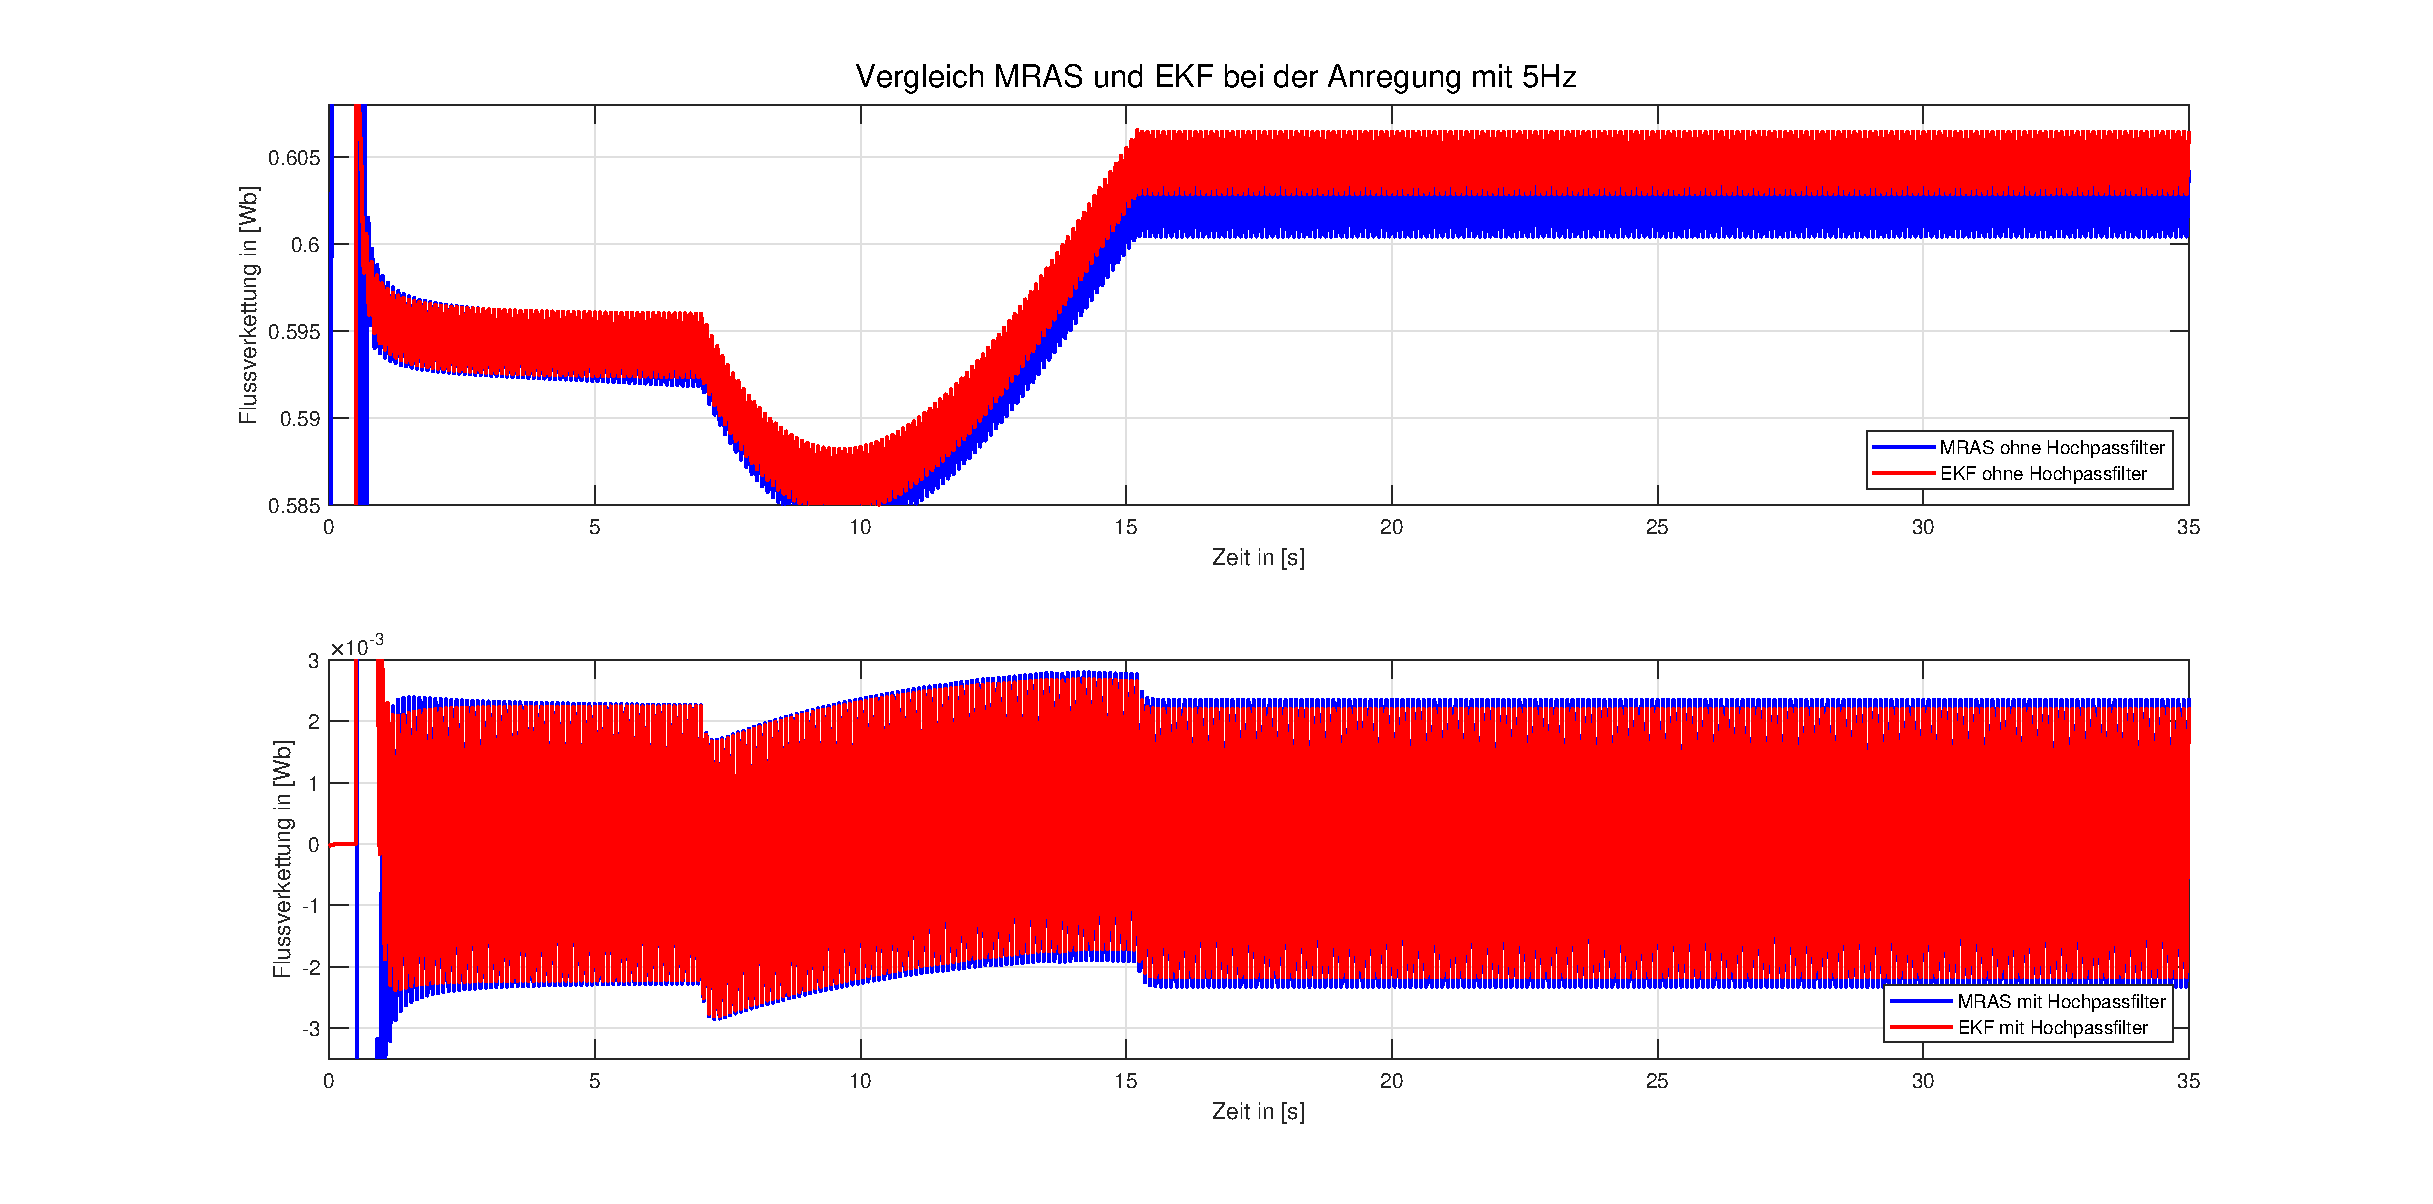
\includegraphics[scale=0.30]{Abbildungen/Vergleich_5Hz.eps}
		
	\end{figure}	
	
\end{frame}
%%%%%%%%%%%%%%%%%%%%%%%%%%%%%%%%%%%%%%%%%%%%%%%%%%%%%%%%%%%%%%%%%%%%%%%%%
\begin{frame}
	\frametitle{Vergleich MRAS und EKF ber der Anregung mit 5Hz sinusförmiger Schwingung im Zeitraum 20s bis 25s }
	
	\begin{figure}[htbp]
		\centering
		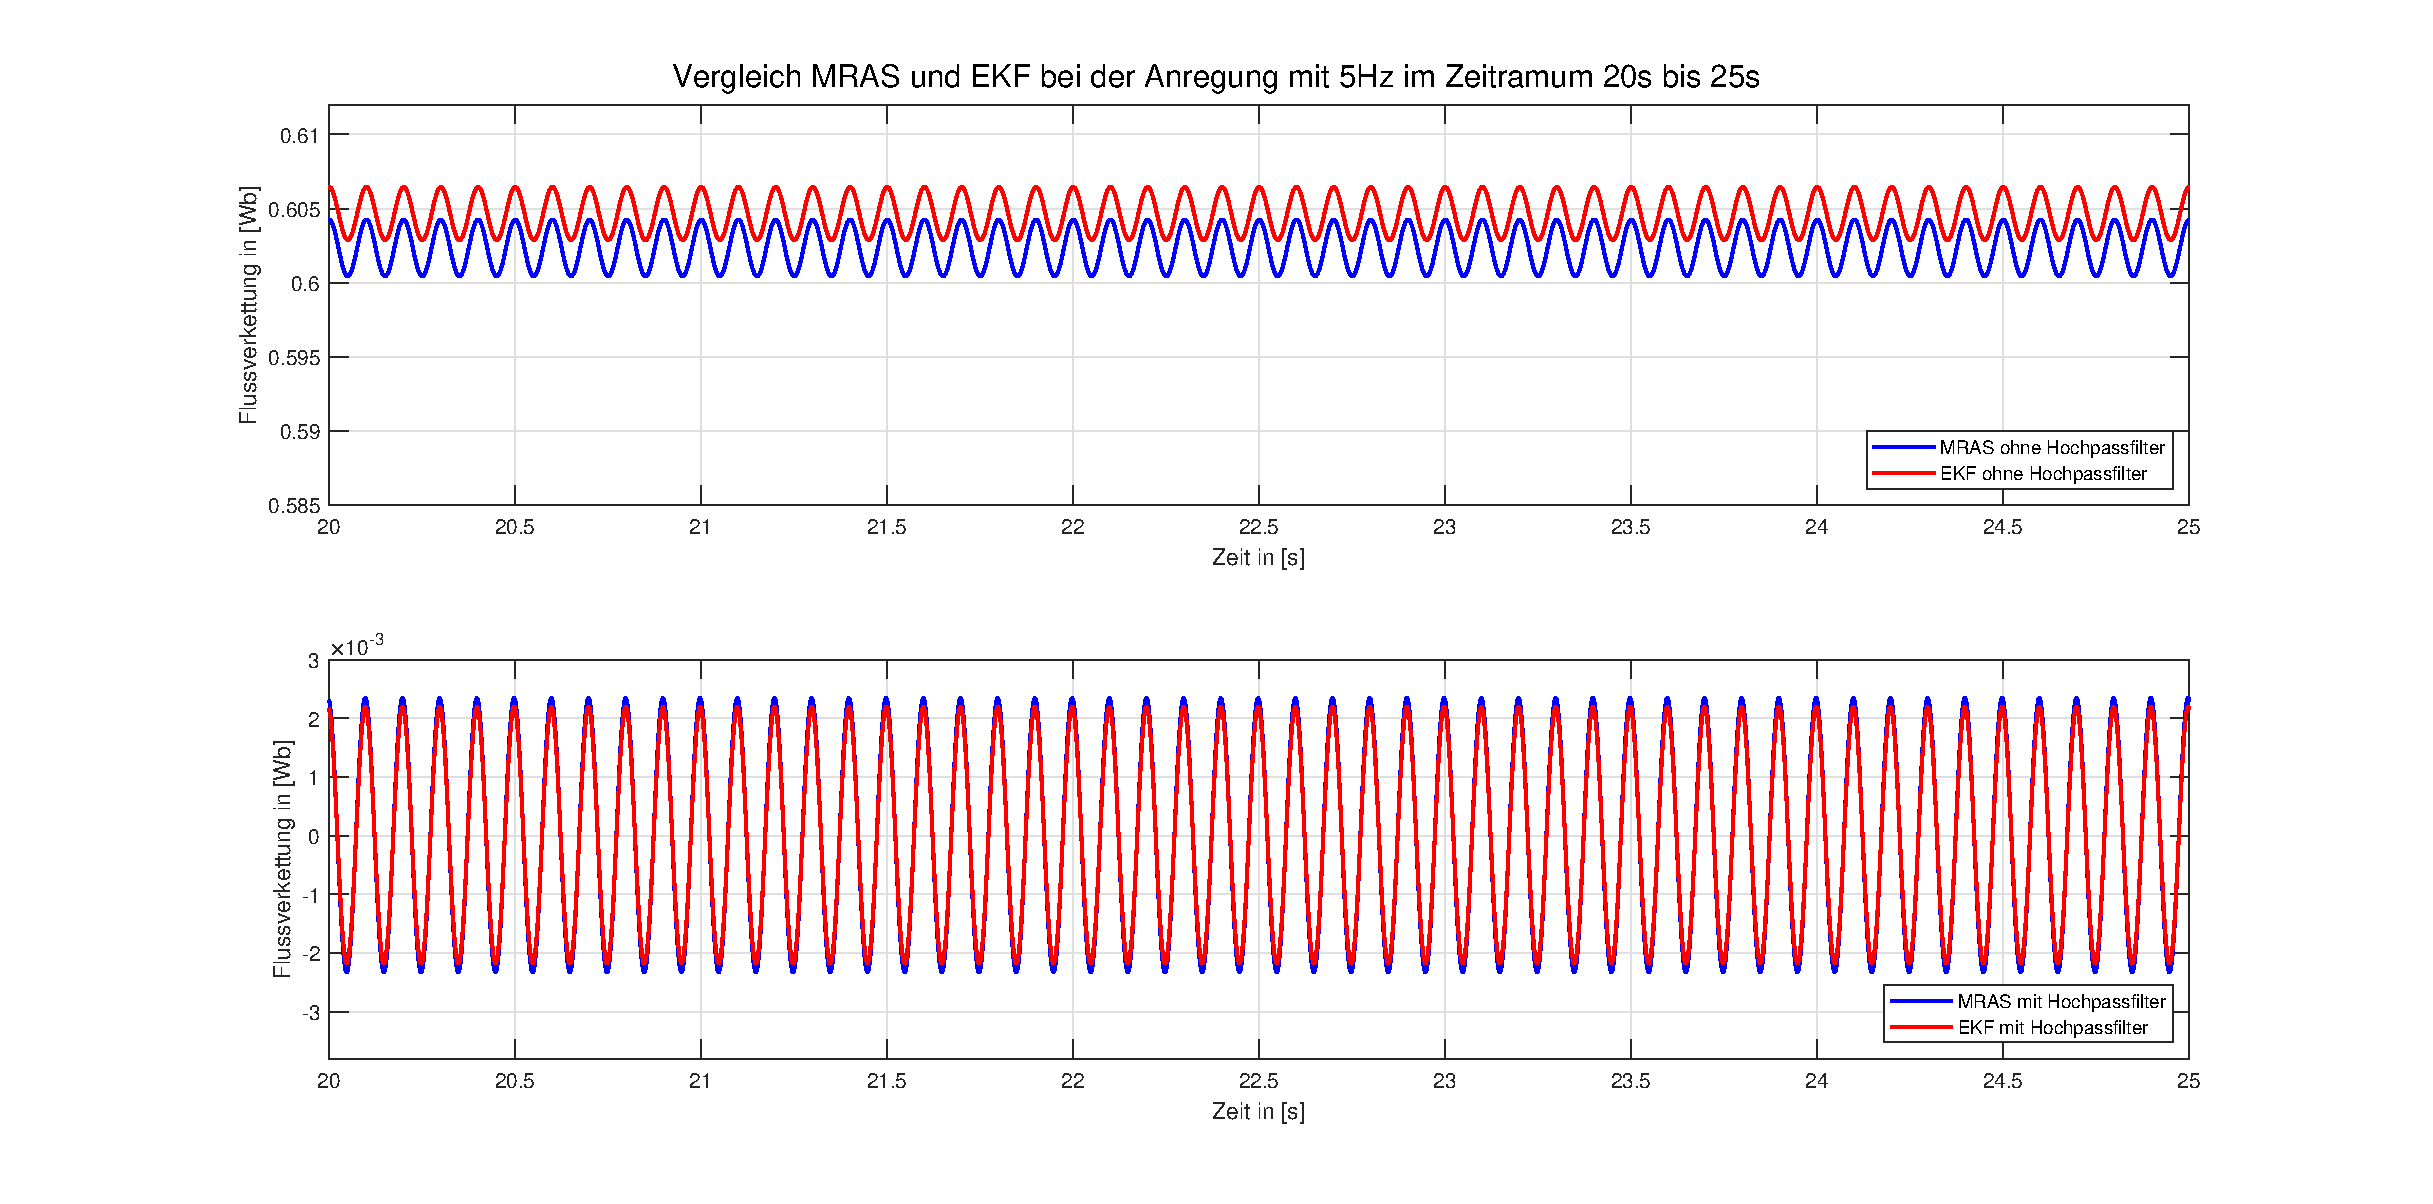
\includegraphics[scale=0.30]{Abbildungen/Vergleich_5Hz_20s.eps}
		
	\end{figure}	
	
\end{frame}
%%%%%%%%%%%%%%%%%%%%%%%%%%%%%%%%%%%%%%%%%%%%%%%%%%%%%%%%%%%%%%%%%%%%%%%%%
\begin{frame}
		\frametitle{Anregung mit 0.1Hz sinusförmige Schwingung beim RLS}
		 
		\begin{figure}[htbp]
			\centering
			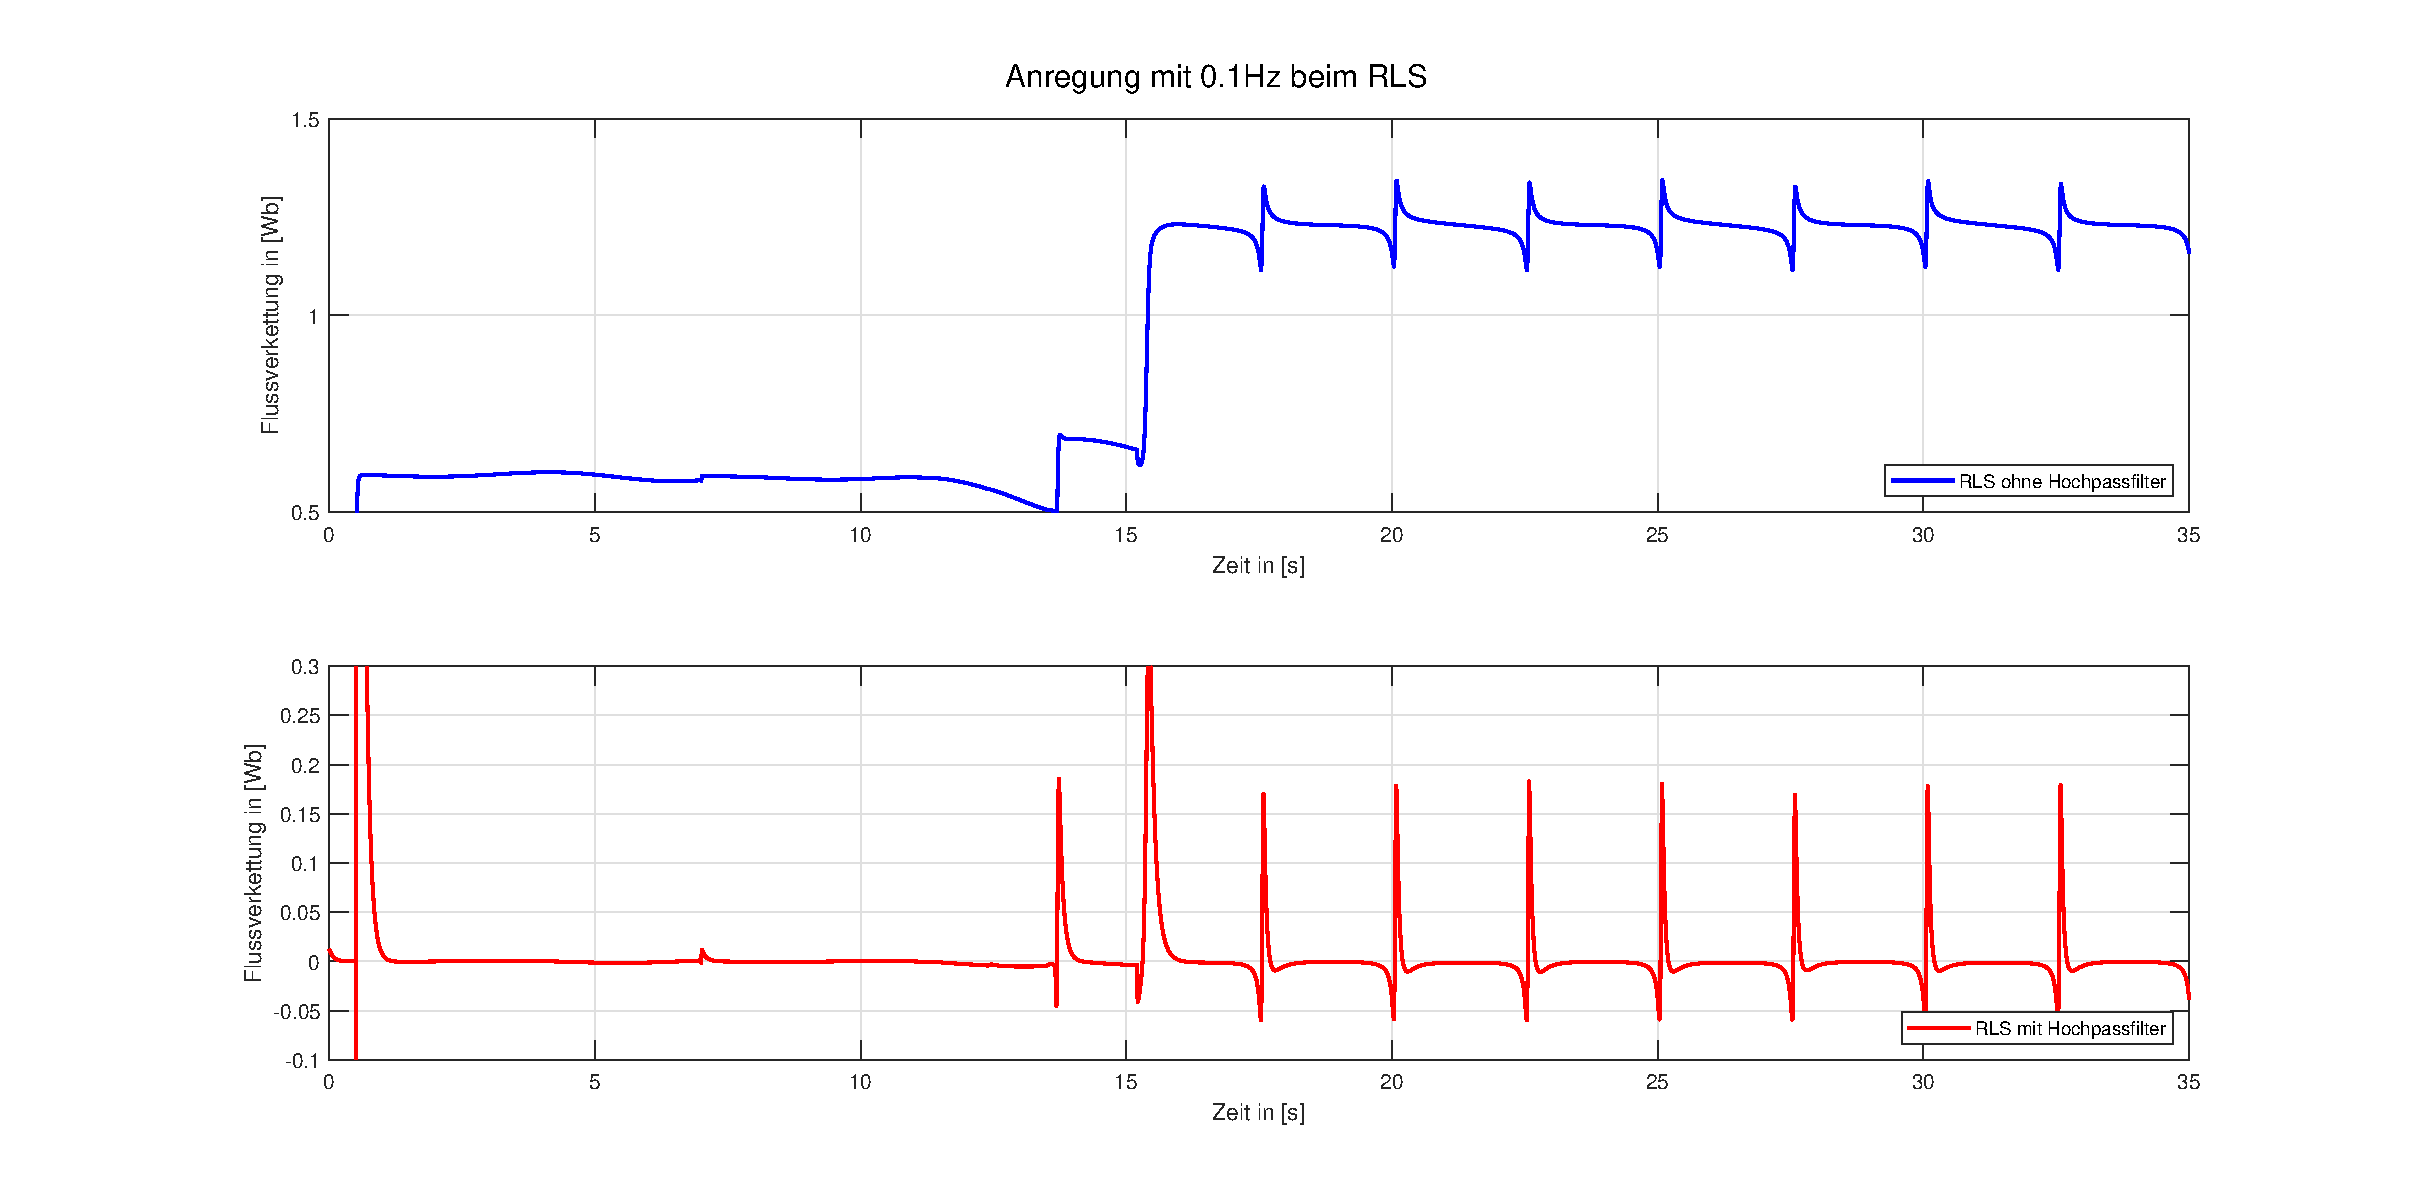
\includegraphics[scale=0.30]{Abbildungen/RLS_01.eps}
			
		\end{figure}	
		
	\end{frame}

%%%%%%%%%%%%%%%%%%%%%%%%%%%%%%%%%%%%%%%%%%%%%%%%%%%%%%%%%%%%%%%%%%%%%%%%%
	\begin{frame}
		\frametitle{Anregung mit 1Hz sinusförmige Schwingung beim RLS}
	
		\begin{figure}[htbp]
			\centering
			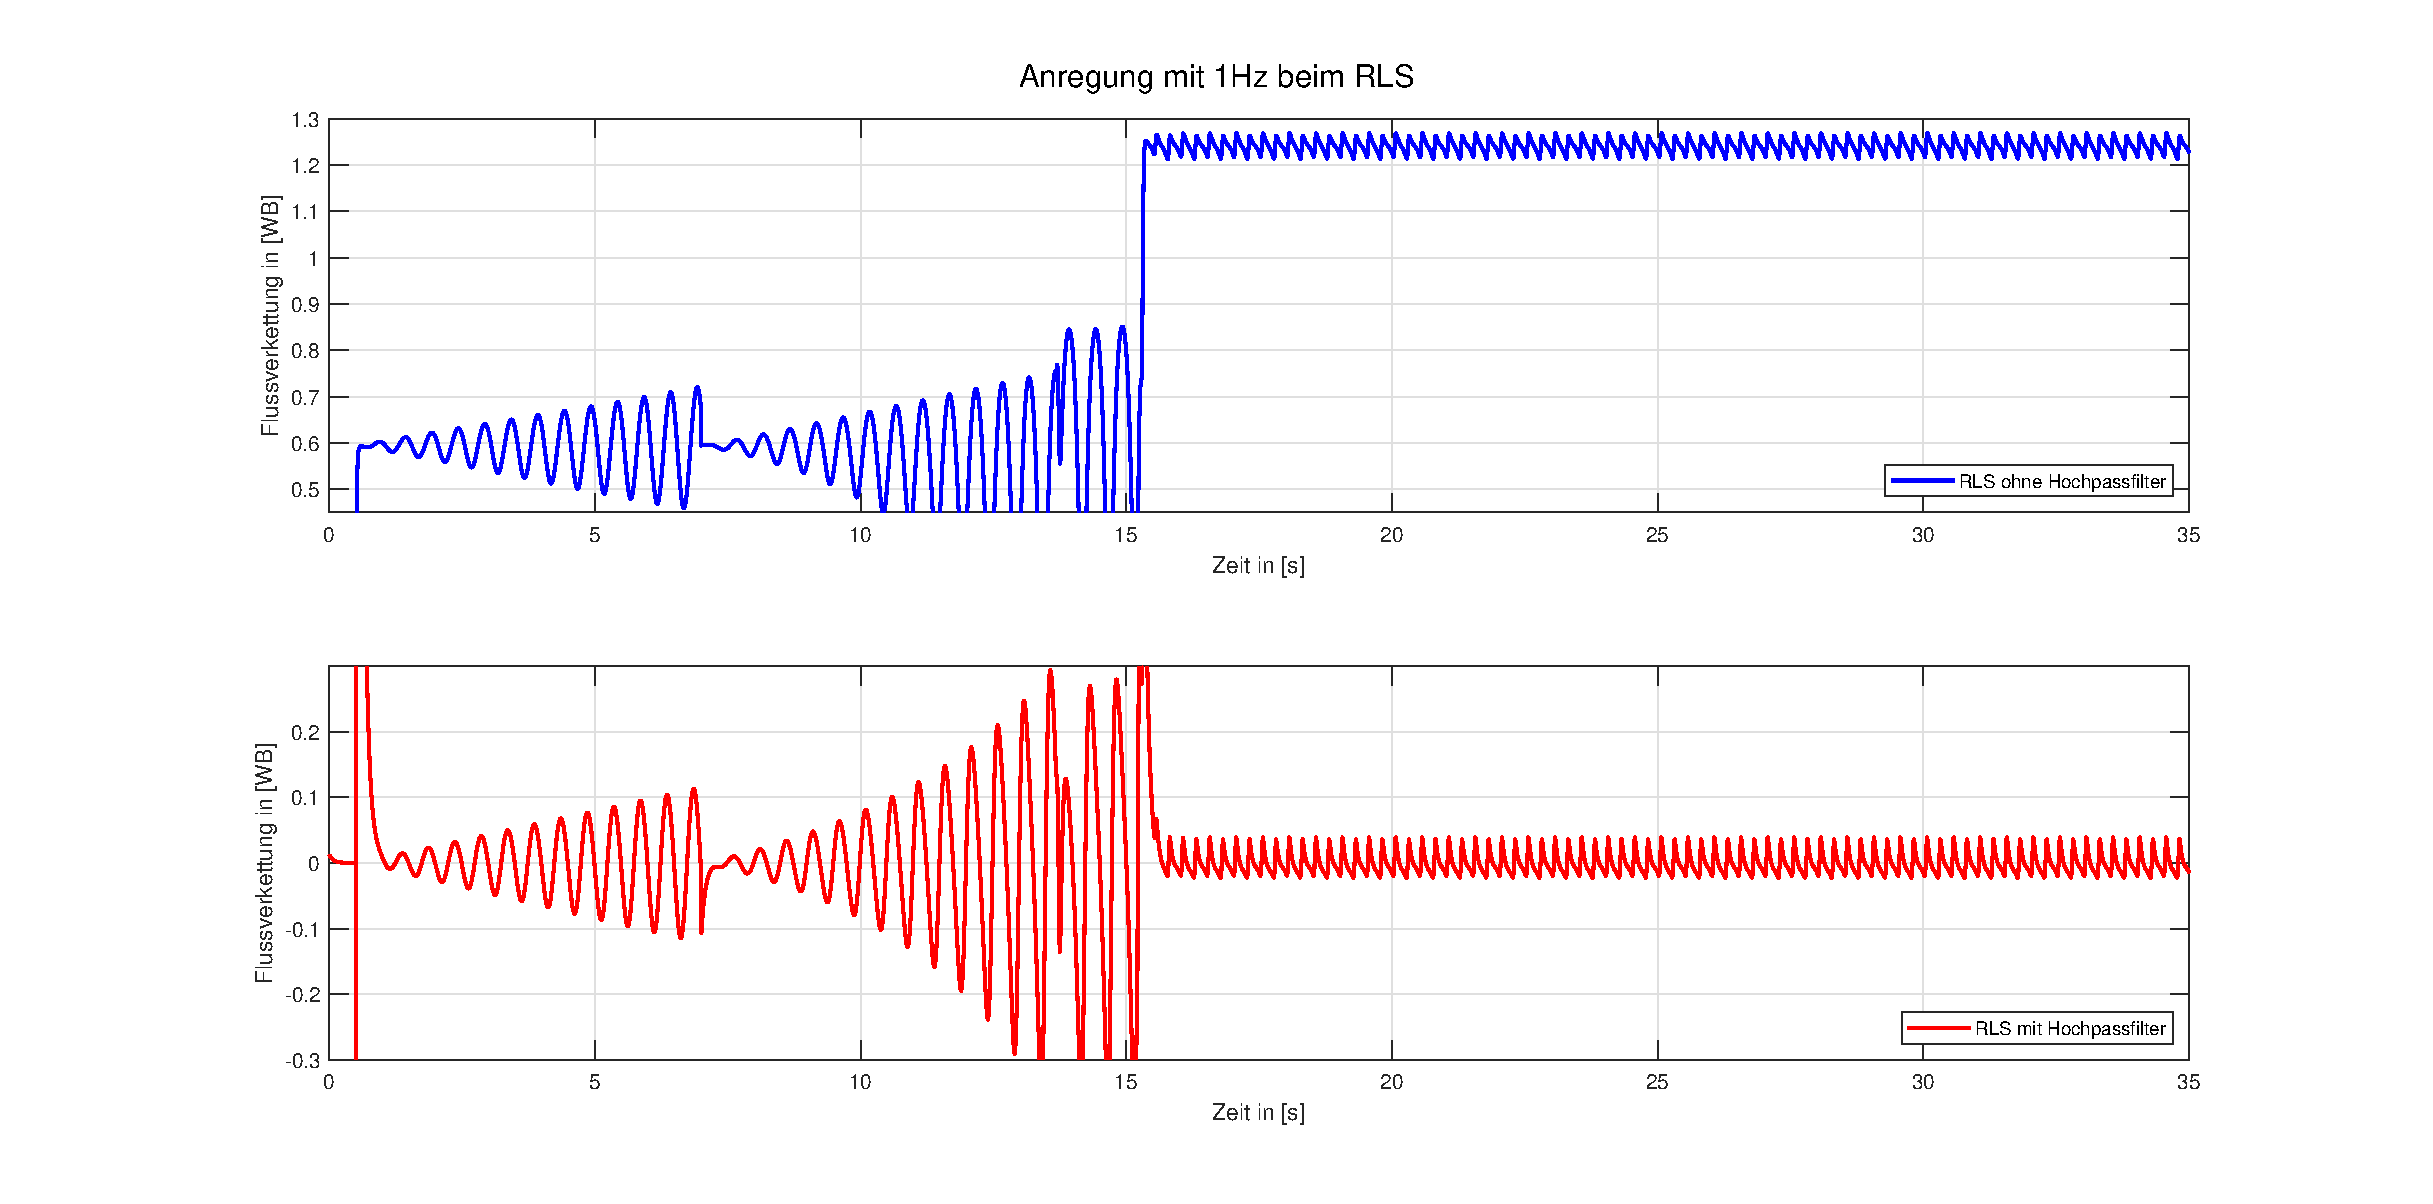
\includegraphics[scale=0.30]{Abbildungen/RLS_1.eps}
			
		\end{figure}	
		
	\end{frame}
	%%%%%%%%%%%%%%%%%%%%%%%%%%%%%%%%%%%%%%%%%%%%%%%%%%%%%%%%%%%%%%%%%%%%%%%%%
	\begin{frame}
		\frametitle{Anregung mit 2Hz sinusförmige Schwingung beim RLS}
		
		\begin{figure}[htbp]
			\centering
			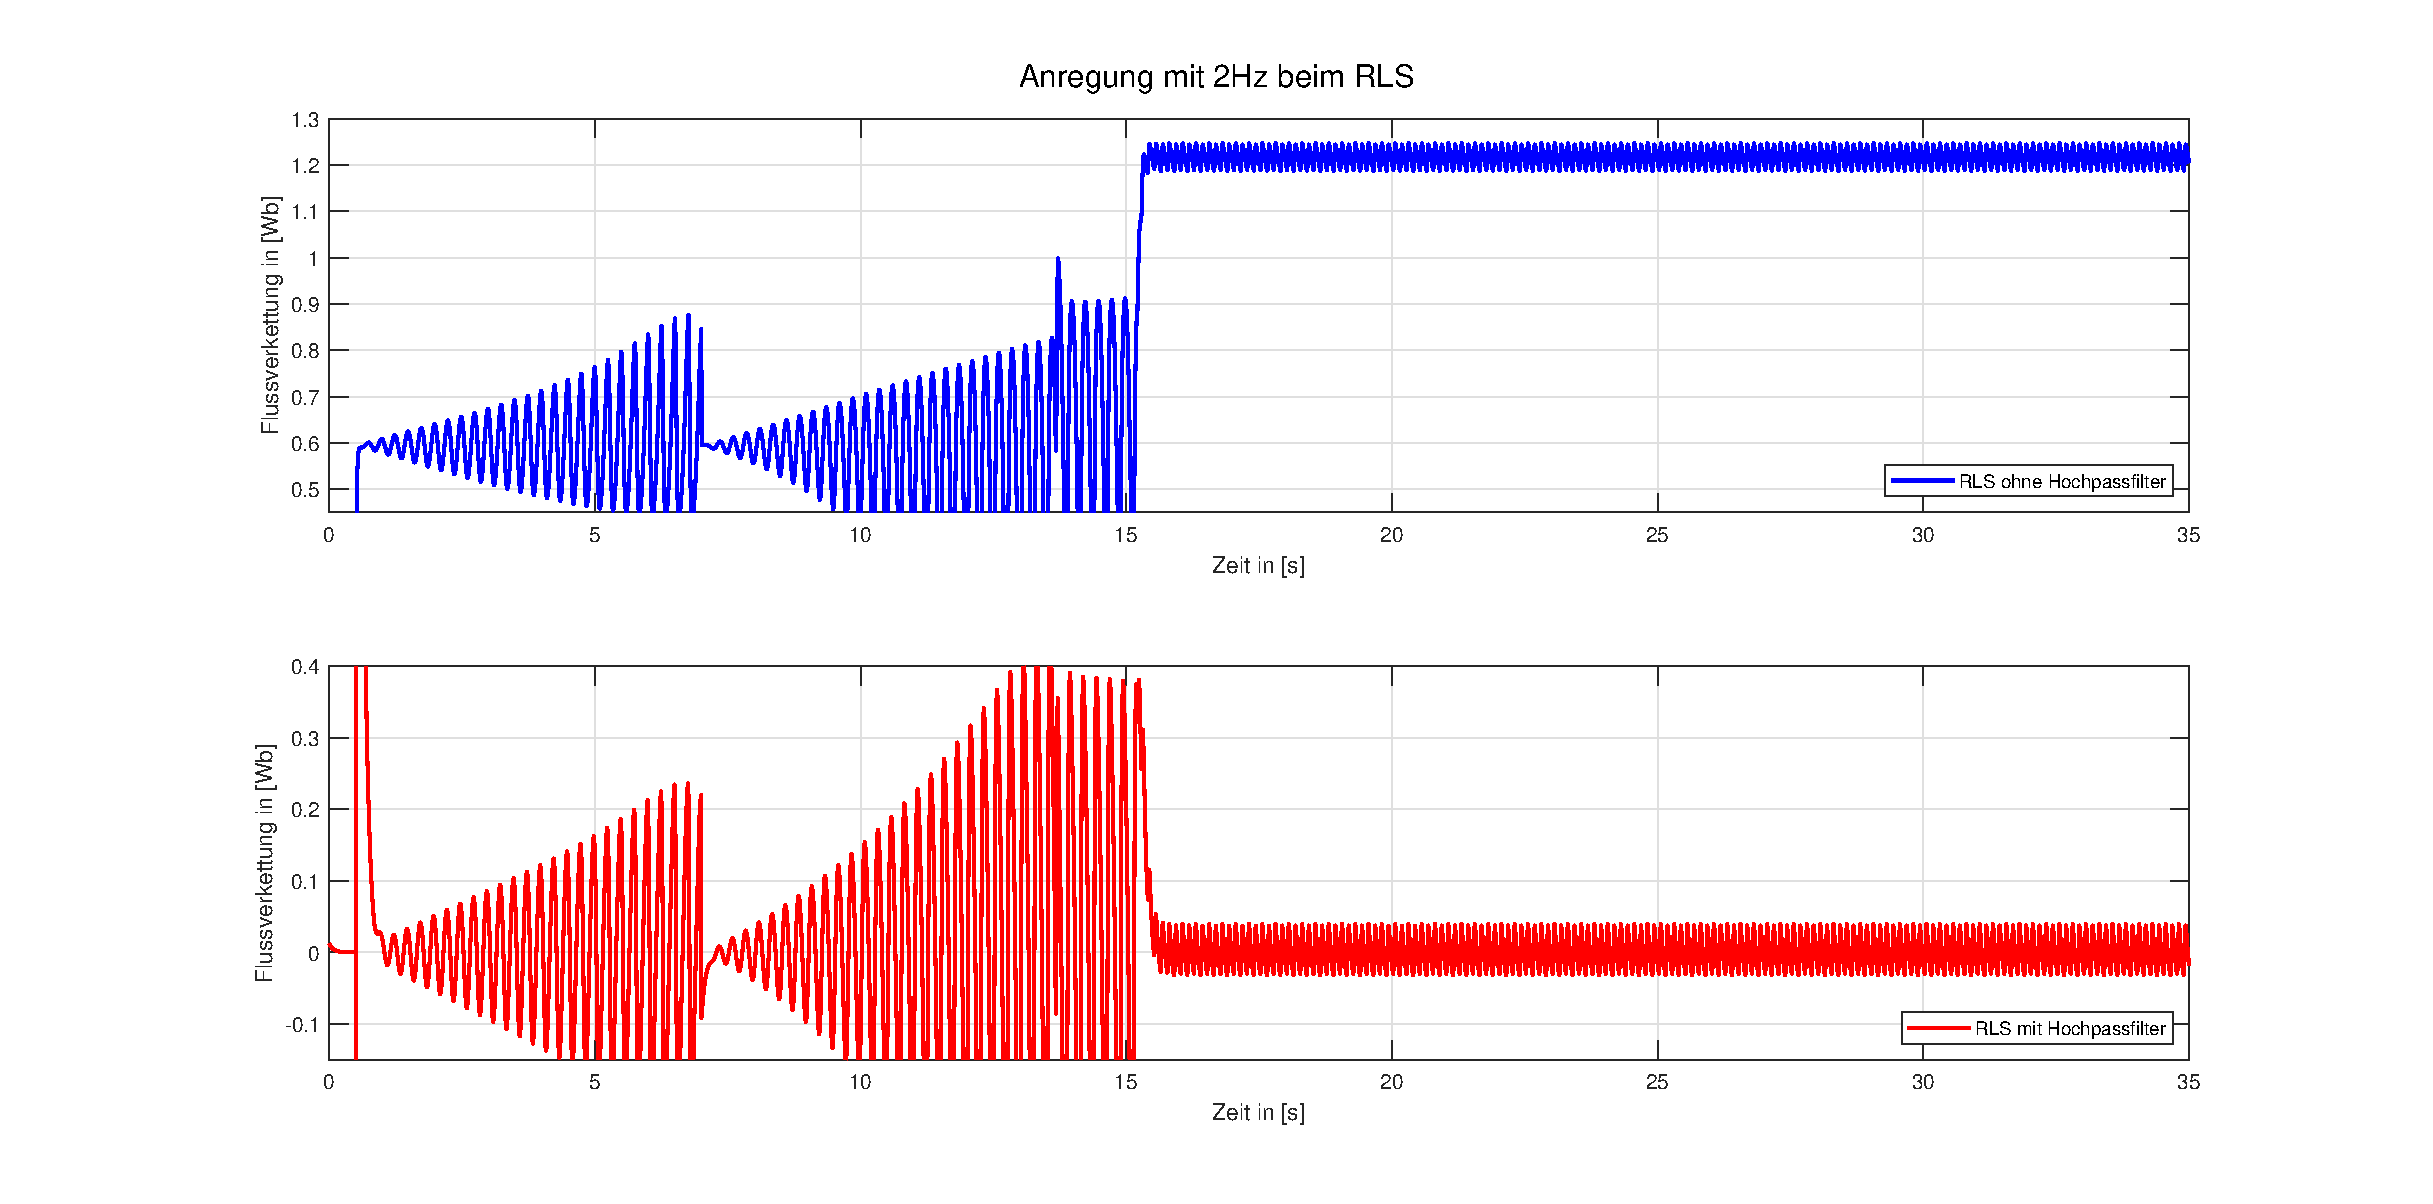
\includegraphics[scale=0.30]{Abbildungen/RLS_2.eps}
			
		\end{figure}	
		
	\end{frame}


%%%%%%%%%%%%%%%%%%%%%%%%%%%%%%%%%%%%%%%%%%%%%%%%%%%%%%%%%%%%%%%%%%%%%%%%%
	\begin{frame}
		\frametitle{Anregung mit 0.1Hz sinusförmige Schwingung beim LB}
		
		\begin{figure}[htbp]
			\centering
			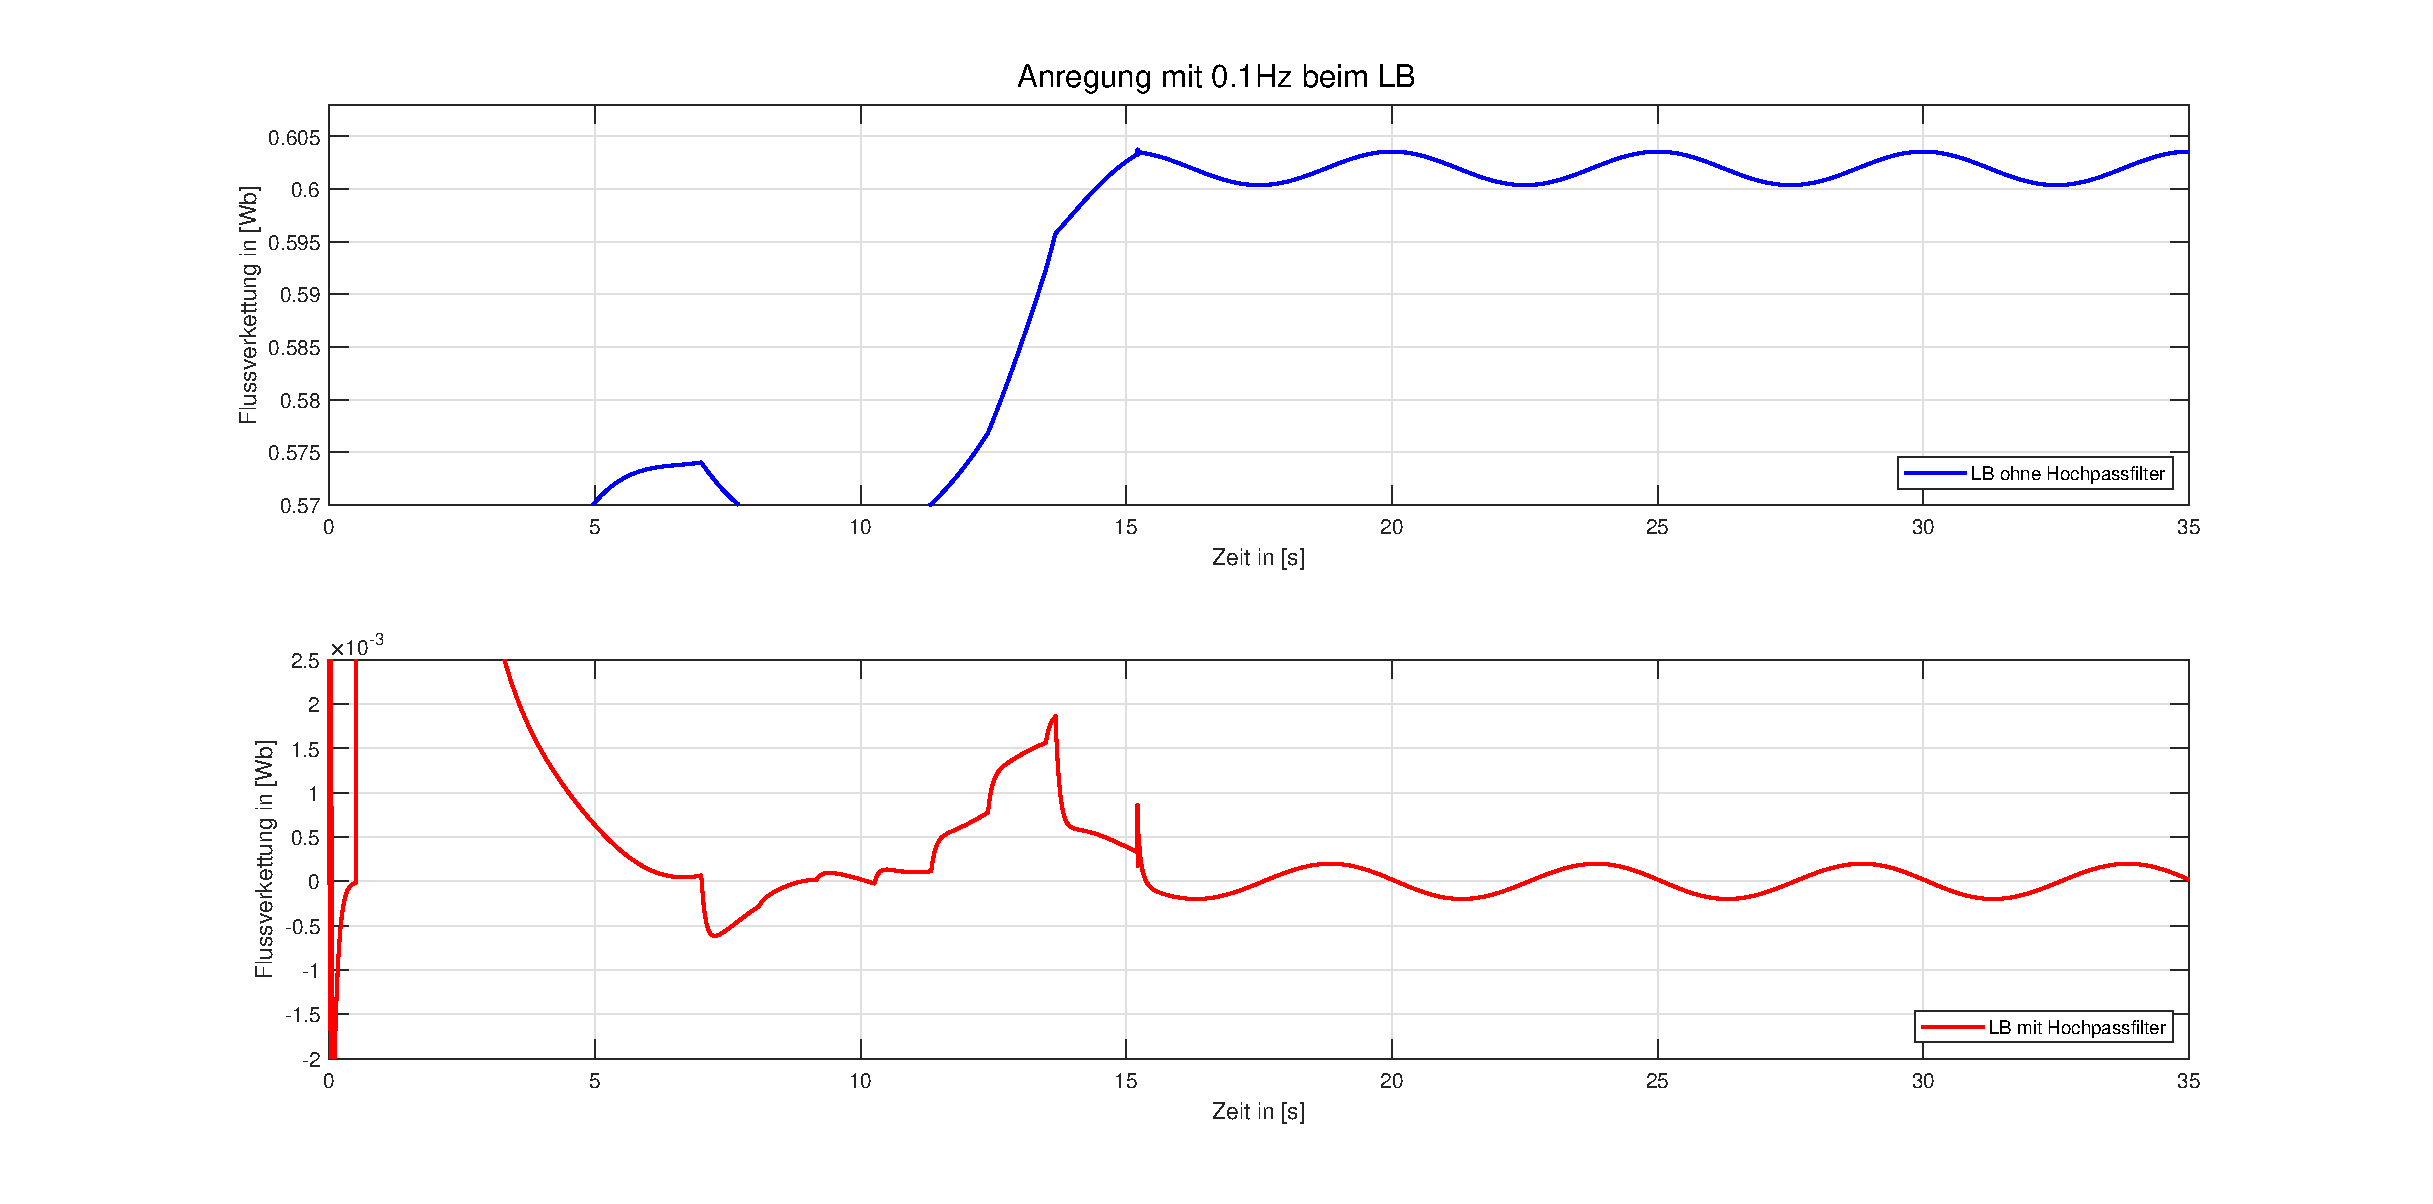
\includegraphics[scale=0.30]{Abbildungen/LB_01.eps}
			
		\end{figure}	
		
	\end{frame}
	%%%%%%%%%%%%%%%%%%%%%%%%%%%%%%%%%%%%%%%%%%%%%%%%%%%%%%%%%%%%%%%%%%%%%%%%%
	\begin{frame}
		\frametitle{Anregung mit 1Hz sinusförmige Schwingung beim LB}
		
		\begin{figure}[htbp]
			\centering
			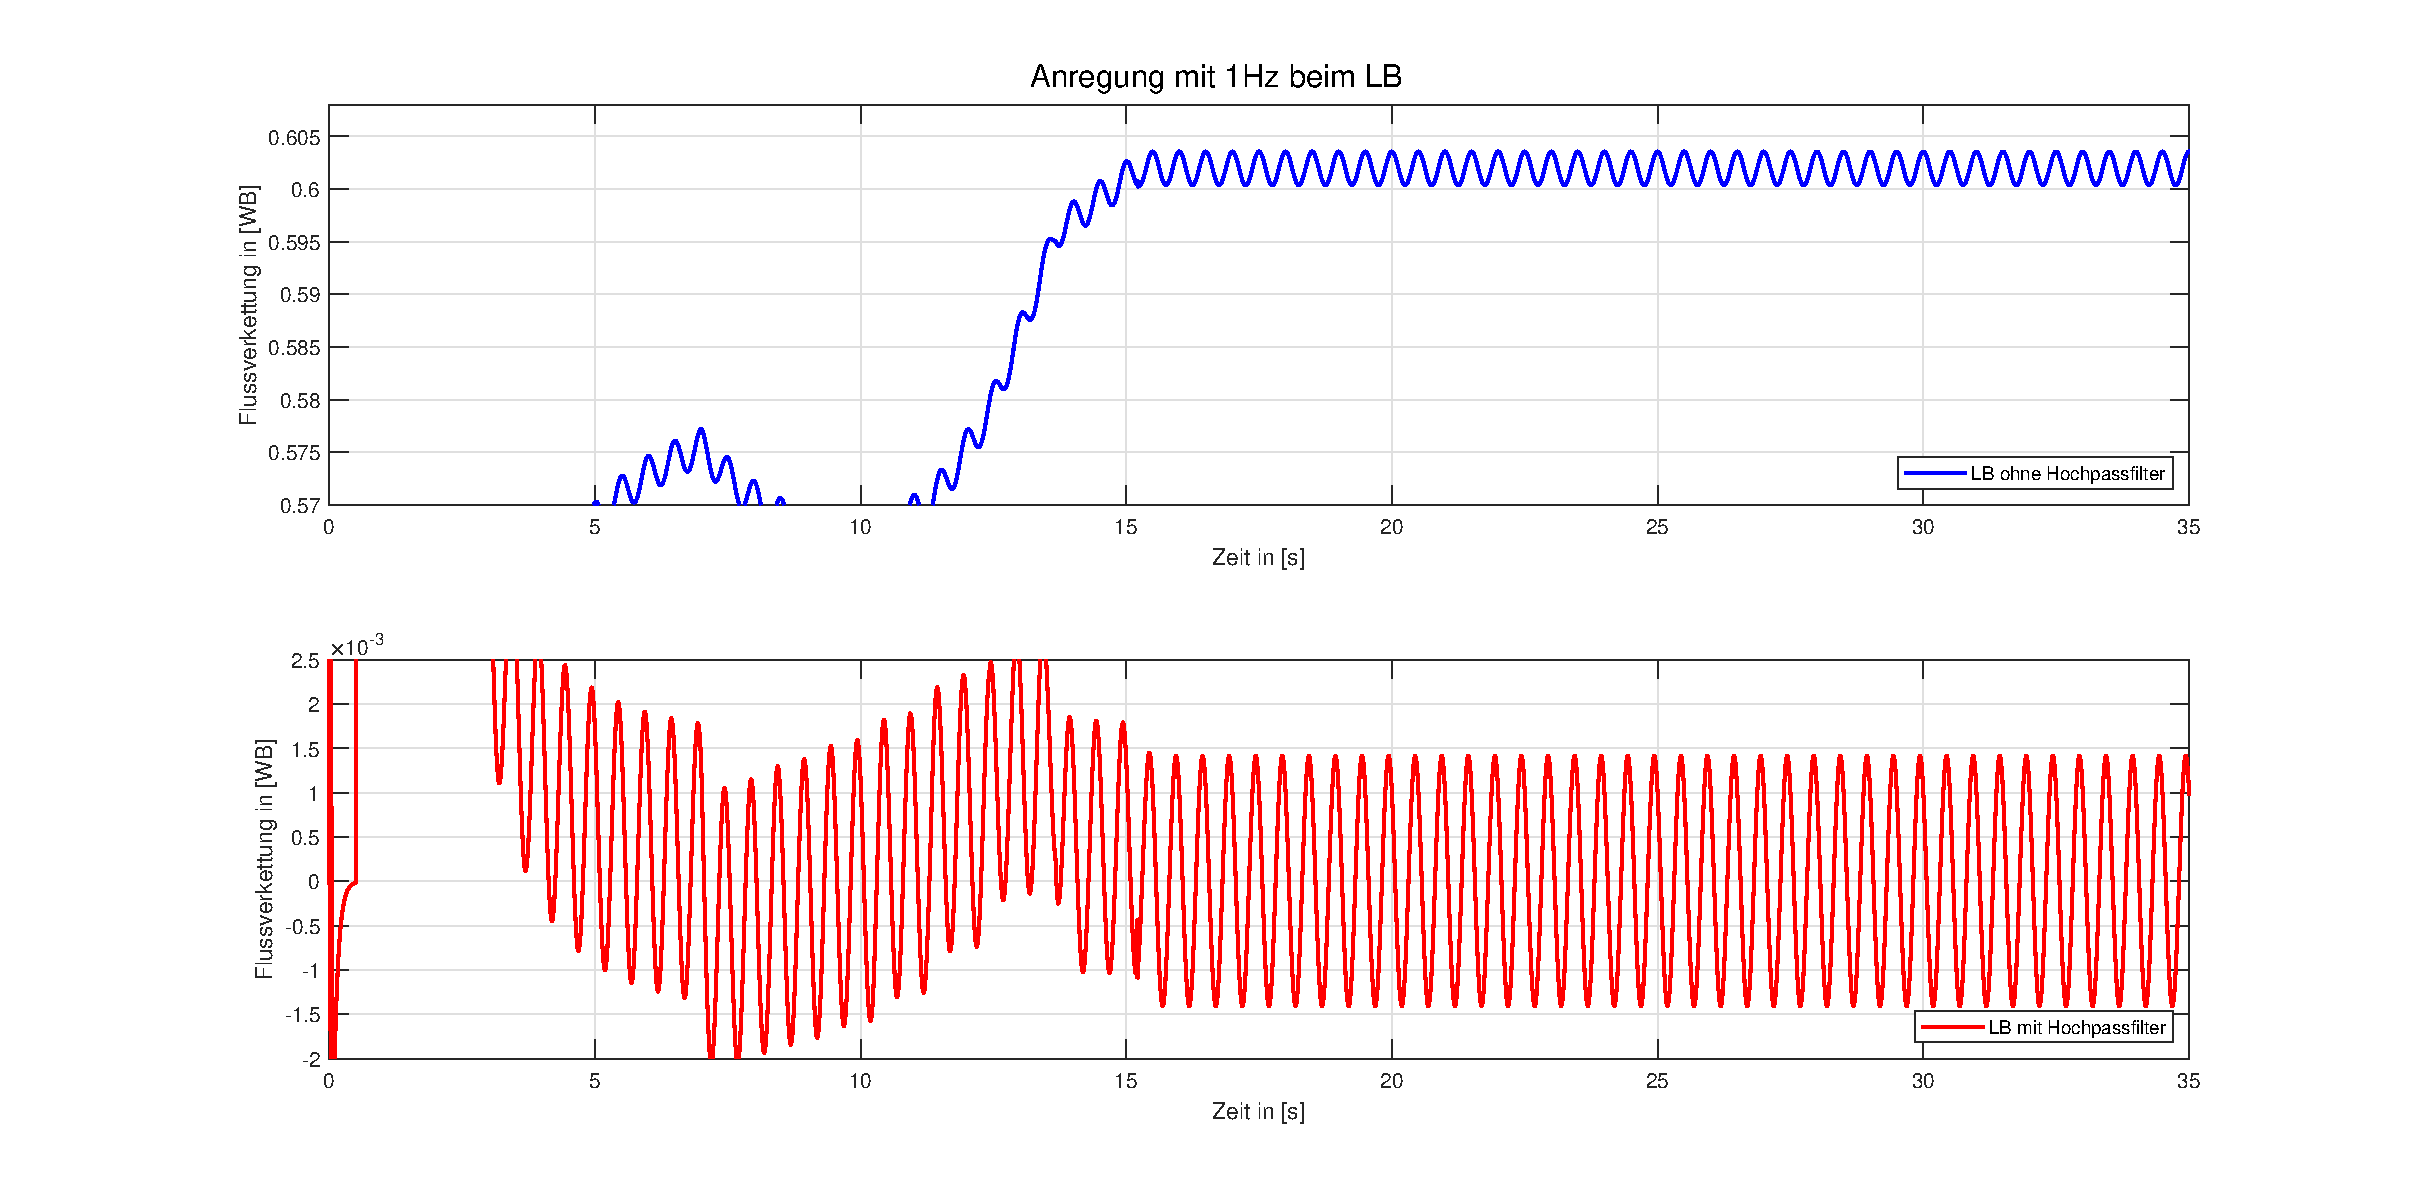
\includegraphics[scale=0.30]{Abbildungen/LB_1.eps}
			
		\end{figure}	
		
	\end{frame}
	%%%%%%%%%%%%%%%%%%%%%%%%%%%%%%%%%%%%%%%%%%%%%%%%%%%%%%%%%%%%%%%%%%%%%%%%%
	\begin{frame}
		\frametitle{Anregung mit 2Hz sinusförmige Schwingung beim LB}
	
		\begin{figure}[htbp]
			\centering
			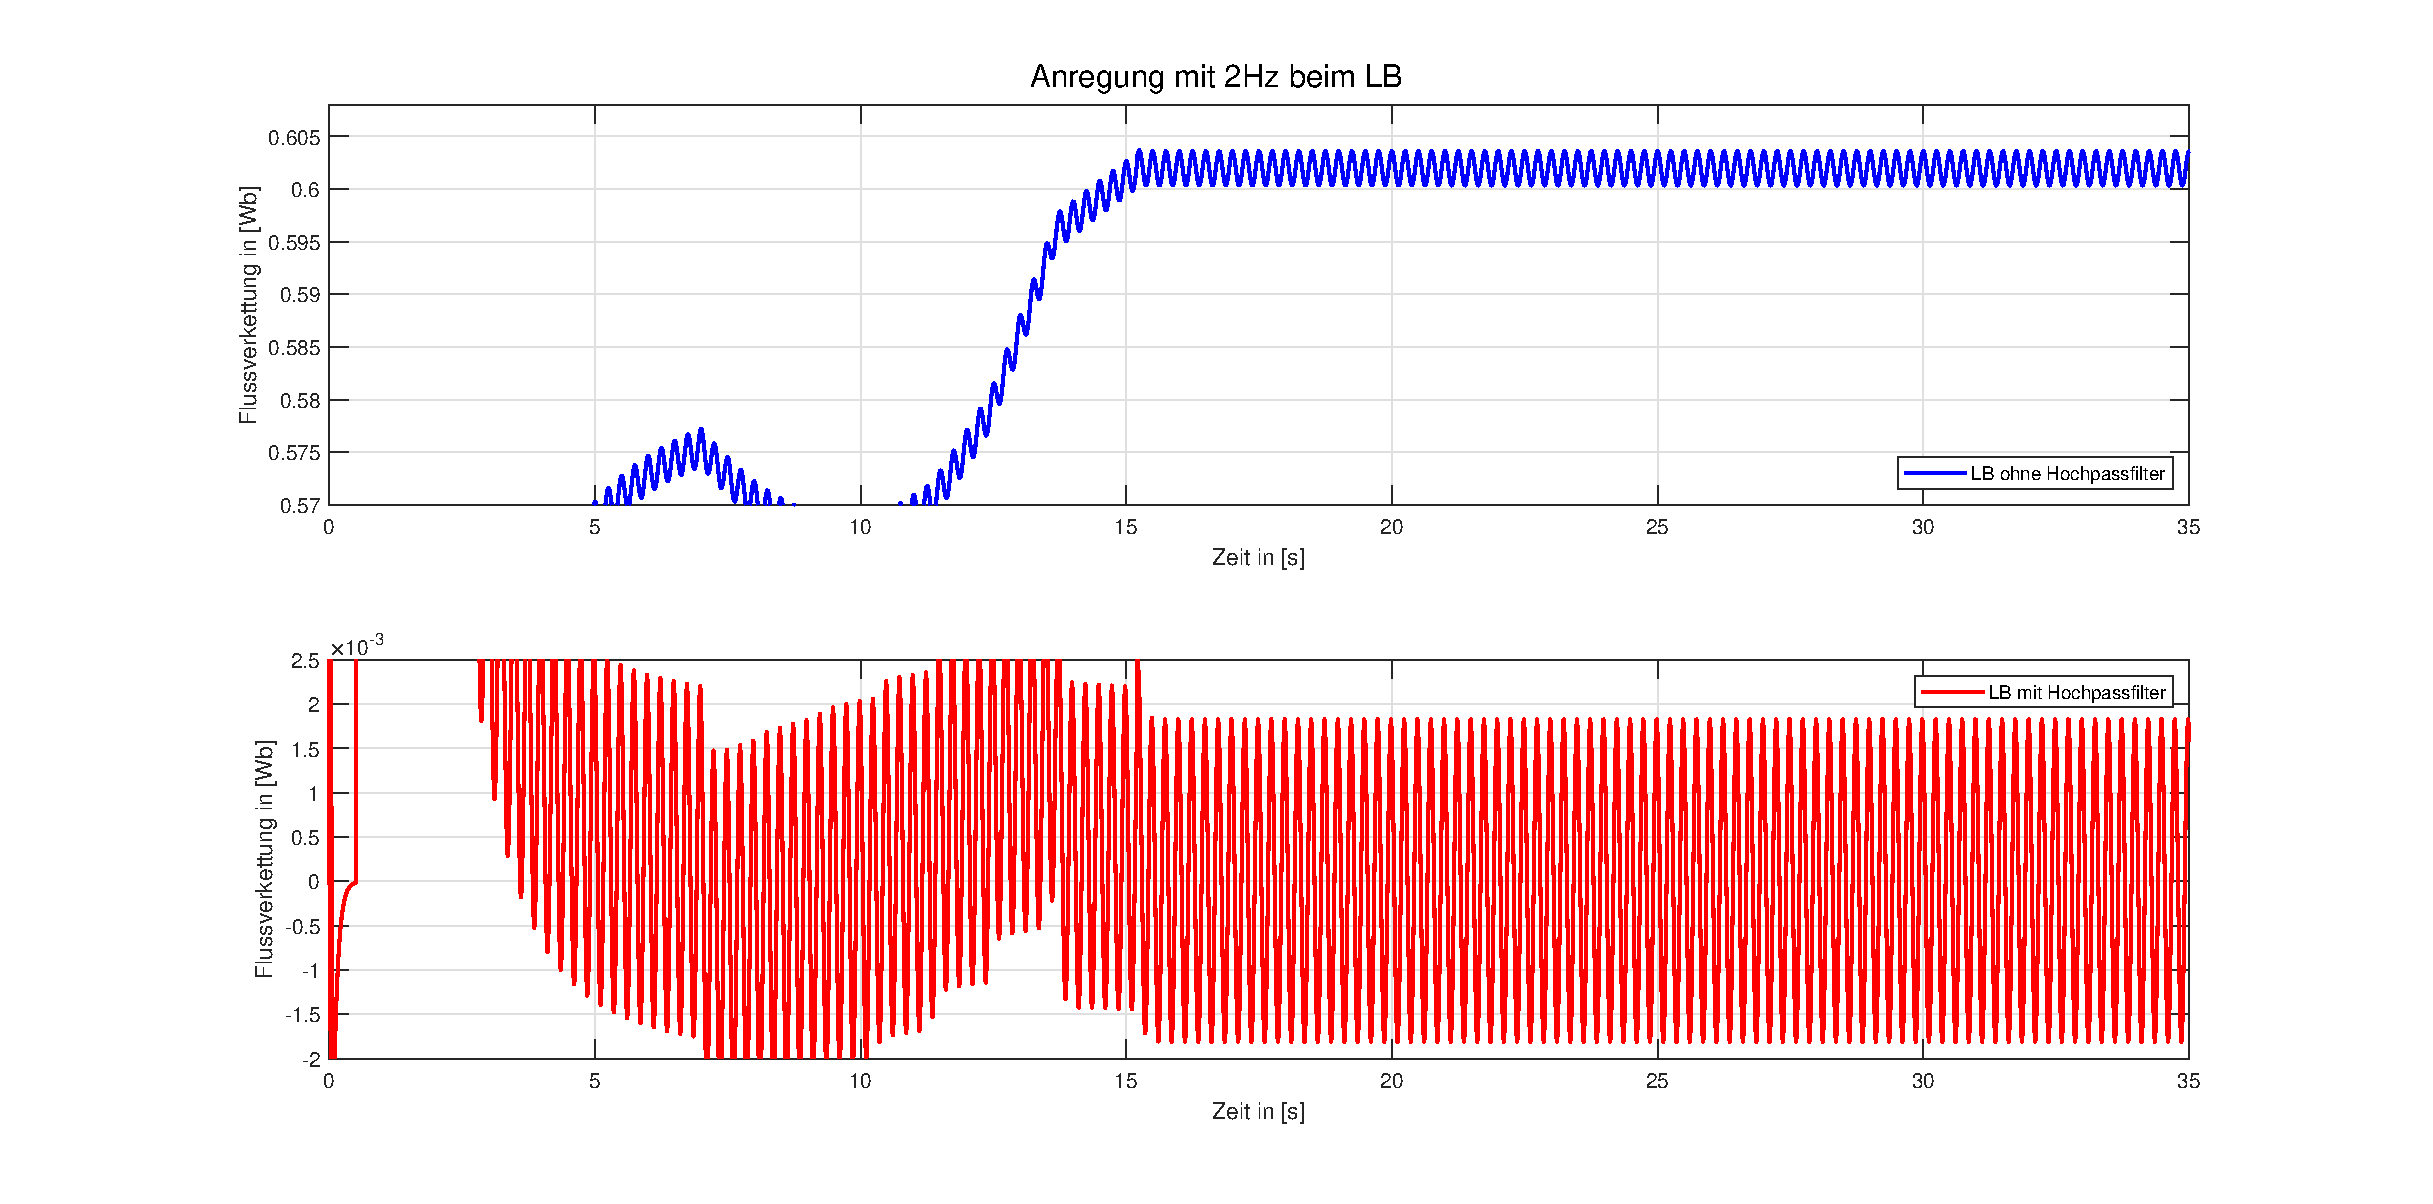
\includegraphics[scale=0.30]{Abbildungen/LB_2.eps}
			
		\end{figure}	
		
	\end{frame}
	%%%%%%%%%%%%%%%%%%%%%%%%%%%%%%%%%%%%%%%%%%%%%%%%%%%%%%%%%%%%%%%%%%%%%%%%%
	\section{Verifizierungsphase}

\begin{frame}
		\frametitle{Verifizierung der Methoden zur Parameterschätzung}
Aus das Ergebnis von Simulation wird die Konzepte \\
		\begin{itemize}
			\item MRAS
			
			\item EKF
		\end{itemize}
an einem Demonstrator innerhalb einer Laborumgebung verifizieren.		
			\begin{figure}[htbp]
			\centering
			\begin{minipage}[t]{0.45\textwidth}
				\centering
				\includegraphics[width=5cm]{Abbildungen/Teststand.JPG}
				
			\end{minipage}
			\begin{minipage}[t]{0.48\textwidth}
				\centering
				\includegraphics[width=5cm]{Abbildungen/Teststand2.JPG}
				
			\end{minipage}
		\end{figure}	
		
	\end{frame}
%%%%%%%%%%%%%%%%%%%%%%%%%%%%%%%%%%%%%%%%%%%%%%%%%%%%%%%%%%%%%%%%%%%%%%%%%
	\section{Abschluss}
	\begin{frame}
		
		\Large{\centerline{Vielen Dank für Ihre Aufmerksamkeit!}}
		
	\end{frame}
%%%%%%%%%%%%%%%%%%%%%%%%%%%%%%%%%%%%%%%%%%%%%%%%%%%%%%%%%%%%%%%%%%%%%%%%%
%\begin{frame}
%	\begin{itemize}
%		\item Frage über Modell für EKF
%	\end{itemize}  
	
%	\begin{floatingfigure}[r]{0.38\linewidth}
%		\includegraphics[scale=0.46]{Abbildungen/Fluxdq.JPG}
		
%	\end{floatingfigure}
%	 \vskip 0.2cm
%	$$\left\{\begin{array}{l}
%		\frac{di_{d}}{dt}=-\frac{R_{s}}{L_{d}}\cdot i_{d}+\frac{\omega L_{q}}{L_{d}}\cdot i_{q}+\frac{U_{d}}{L_{d}}+\frac{\omega}{L_{d}}\cdot \psi_{rq}\\
%		\frac{di_{d}}{dt}=-\frac{R_{s}}{L_{d}}\cdot i_{d}+\frac{\omega L_{q}}{L_{d}}\cdot i_{q}+\frac{U_{d}}{L_{d}}
%		\\\frac{di_{q}}{dt}=-\frac{R_{s}}{L_{q}}\cdot i_{q}-\frac{\omega L_{d}}{L_{q}}\cdot i_{d}+\frac{U_{q}}{L_{q}}-\frac{\omega}{L_{q}}\cdot \psi_{rd}\\
%		\frac{di_{q}}{dt}=-\frac{R_{s}}{L_{q}}\cdot i_{q}-\frac{\omega L_{d}}{L_{q}}\cdot i_{d}+\frac{U_{q}}{L_{q}}-\frac{\omega}{L_{q}}\psi_{f}\\
%	\end{array}\right.$$
%	\end{frame}

%%%%%%%%%%%%%%%%%%%%%%%%%%%%%%%%%%%%%%%%%%%%%%%%%%%%%%%%%%%%%%%%%%%%%%%%%	


\end{document}